\documentclass[ASNA,twocolumn]{USG}
\usepackage{anyfontsize}
\usepackage{xcolor}
\usepackage{booktabs}
\usepackage{siunitx}
\usepackage{amsmath}
\usepackage{algorithm}
\usepackage{algpseudocode}
\usepackage{longtable}
\graphicspath{{./images/}{../../figures/}}
\makeatletter
% article-type banner without the open-access badge of the template sample
\def\@@articletype{\rule[-4\p@]{4\p@}{15\p@}{\arttypefont\bf\uppercase{\letterspace to 1.15\naturalwidth{\@articletype}}}}
\makeatother

\specialissue{AI and Remote Sensing for Environmental Geosciences: Data-Driven Approaches to Geology, Environmental Processes and Natural Hazards}
\articletype{ORIGINAL ARTICLE}
\journal{New Zealand Journal of Geology and Geophysics}
\volume{0}
\copyyear{2026}
\startpage{1}
\articledoi{10.1002/0000}

\begin{document}

\title{Transferable coseismic landslide forecasting across the Pacific Rim with hierarchical physics-anchored boosting and selection-aware Bayesian updating}

\author[1]{Quang-Vinh Dang}[https://orcid.org/0000-0002-3877-8024]
\author[2]{Dat Le}[https://orcid.org/0009-0005-5038-8570]
\author[3]{Minh Ngoc Dinh}[https://orcid.org/0000-0003-4026-6068]

\authormark{DANG \textsc{et al.}}
\titlemark{TRANSFERABLE COSEISMIC LANDSLIDE FORECASTING ACROSS THE PACIFIC RIM}

\address[1]{\orgname{British University Vietnam, }\orgaddress{\state{Hung Yen, }\country{Vietnam}}}
\address[2]{\orgdiv{Department of Science, Technology, and International Projects, }\orgname{Ho Chi Minh City University of Economics and Finance, }\orgaddress{\state{Ho Chi Minh City 700000, }\country{Vietnam}}}
\address[3]{\orgdiv{Data Science and Information Technology, }\orgname{Millennia University, }\orgaddress{\state{Ho Chi Minh City, }\country{Vietnam}}}

\corres{Minh Ngoc Dinh (\email{minh.dinh@maeducation.com})}
\presentaddress{Submitting author: Quang-Vinh Dang (\email{vinh.dq4@buv.edu.vn}), British University Vietnam, Hung Yen, Vietnam.}

\fundingInfo{This research received no specific grant from any funding agency.}

\keywords{coseismic landslides | transfer learning | physics-informed machine learning | Bayesian updating | Newmark displacement | Kaik\={o}ura earthquake | Pacific Rim | ShakeMap}

\abstract[ABSTRACT]{We test how well coseismic landslide models trained on past earthquakes transfer to unseen ones, first across nine Pacific Rim events with open inventories, including Kaik\={o}ura 2016, then across 38 earthquakes worldwide, using only rapidly available inputs: Copernicus GLO-30 terrain, USGS ShakeMap ground motion and Newmark sliding-block displacement. Physics-based, logistic and gradient-boosting models rank hillslopes reasonably well in an unseen earthquake but mispredict its total amount of landsliding by up to three orders of magnitude, mostly as a shift in level rather than in shape. We therefore propose HiPhyBoost (hierarchical physics-anchored boosting). It combines (i) a Newmark-anchored, monotone-constrained boosted model with latent event offsets, (ii) an empirical-Bayes prior over offsets that yields zero-shot predictive intervals for the landslide total, and (iii) a quasi-likelihood Bayesian update of the offset from a few rapidly mapped image tiles that accounts for landslide clustering. Across 38 earthquakes, HiPhyBoost transferred better than physics-constrained boosting in 29 events (median AUC 0.795 against 0.763; mean gain 0.013), including 21 of 29 events not used in its development. It reached AUC 0.917 for Kaik\={o}ura without New Zealand training data. After one to ten mapped tiles it predicted the remaining landslide total within a median factor of 1.4--1.6, with far better calibrated intervals than a pixel-independent update. The event offsets summarise each earthquake's landslide propensity relative to generic slope mechanics but also reflect how inventories were mapped. Offsets tended to be higher after wetter-than-normal months over the shaken area, and conditioning the prior on covariates available at forecast time (magnitude, depth, mechanism, ShakeMap station count, antecedent wetness) narrowed zero-shot intervals more than threefold without loss of coverage, but did not improve point forecasts. For Aotearoa New Zealand, the results support issuing Alpine Fault or Hikurangi scenario forecasts as intervals and planning rapid tile mapping to narrow them.}

\maketitle

\section{Introduction}\label{sec:intro}

Strong earthquakes in steep, tectonically active terrain trigger thousands to tens of thousands of landslides within seconds. These landslides cause a large share of earthquake fatalities, cut transport corridors and start sediment cascades that persist for years \citep{keefer1984,fan2019}. The 2016 M\textsubscript{w}~7.8 Kaik\={o}ura earthquake ruptured more than twenty faults \citep{hamling2017} and triggered roughly 30\,000 landslides over about \SI{10000}{\square\kilo\metre} of northeastern South Island \citep{massey2018,massey2020update}. A future Alpine Fault earthquake is expected to produce a comparable or larger landslide response in the Southern Alps \citep{robinson2016}, and response planning for that scenario depends on landslide forecasts for an event that has not happened \citep{orchiston2018}. The same problem recurs around the Pacific Rim, from the Andes and Central America to Japan, Alaska, Papua New Guinea and Sulawesi.

In the first hours after an earthquake, no inventory exists for the new event. Landslide models used in emergency response therefore have to be \emph{transferred}: they are fitted to past earthquakes and applied to a new one. Operational near-real-time systems do this with logistic regression on ShakeMap ground motion and global terrain and geology layers \citep{nowicki2014,nowickijessee2018,allstadt2022}. Physics-based alternatives use Newmark rigid sliding-block displacement with generic strength parameters \citep{newmark1965,jibson2000,jibson2007}. In parallel, most landslide studies now use machine-learning (ML) classifiers such as gradient-boosted trees, because these usually give the highest discrimination when trained and tested within one region \citep{merghadi2020,reichenbach2018}. Discrimination inside a single event says little about transfer. Spatially autocorrelated samples inflate random cross-validation scores \citep{brenning2012,roberts2017}, and high scores can coexist with geomorphically implausible maps \citep{steger2016}. A flexible learner can also fit event-specific artefacts, such as inventory mapping protocol, local ShakeMap error or lithology, that do not carry over to the next earthquake.

Cross-event transfer has been tested before. Global models are evaluated on events withheld from fitting \citep{nowicki2014,nowickijessee2018,tanyas2019slope}, and fuzzy and regression models have been carried from one earthquake to another \citep{kritikos2015,li2013lushan}. \citet{lombardo2020chrono} framed this as chrono-validation, and \citet{allstadt2018} evaluated candidate global models against the Kaik\={o}ura inventory. These studies leave four questions open, and they are the gaps this paper addresses.

\begin{enumerate}
\item No controlled, like-for-like comparison exists between physics-based, global-style logistic and ML models under leave-one-event-out validation with identical inputs. It is therefore unknown whether the advantage of ML learners survives transfer to a new earthquake, or whether adding physical knowledge as monotonic constraints \citep{karpatne2017,reichstein2019} improves it.
\item Transfer studies rarely separate \emph{discrimination}, the ranking of hillslopes, from \emph{calibration}, the agreement of predicted probabilities with observed landslide frequencies. Calibration is the property most likely to fail in a new population \citep{vancalster2019}, and probability-based products depend on it \citep{allstadt2022}.
\item The value of the first few landslides mapped from post-event imagery \citep{williams2018,handwerger2022} for updating a transferred model has not been quantified, even though clinical prediction research provides established updating methods \citep{steyerberg2004,janssen2008}.
\item Explainable-AI attributions \citep{lundberg2017,lundberg2020} are increasingly read as evidence of process understanding in landslide studies \citep{dahal2023xai}. Whether these attributions stay the same from one earthquake to the next, which they must if a model has learned process, has not been tested.
\end{enumerate}

We address these gaps with nine coseismic landslide inventories from around the Pacific Rim: Kaik\={o}ura 2016 (New Zealand), Northridge 1994 and Denali 2002 (USA), Niigata-Chuetsu 2004 and Iwate-Miyagi 2008 (Japan), Ays\'en 2007 (Chile), Cinchona 2009 (Costa Rica), Porgera 2018 (Papua New Guinea) and Palu 2018 (Indonesia). We use only globally and rapidly available inputs: Copernicus GLO-30 terrain, which is derived from TanDEM-X radar interferometry \citep{copdem,guth2021}, and USGS ShakeMap ground motion \citep{worden2018}. With these inputs we (i) benchmark five models of increasing flexibility in a leave-one-event-out (LOEO) design, including a physics-constrained gradient-boosting model (PC-GBM) whose response to shaking, slope and Newmark displacement is forced to be monotone; (ii) separate transfer error into discrimination and calibration components; (iii) quantify how many rapidly mapped image tiles are needed to recalibrate a transferred model; and (iv) test whether TreeSHAP attributions are stable across events. Kaik\={o}ura is used throughout as the target case for Aotearoa New Zealand.

\section{Data}\label{sec:data}

\subsection{Coseismic landslide inventories}
We selected nine earthquakes around the Pacific Rim that have openly available, event-wide landslide inventories (Figure~\ref{fig:events}; Table~\ref{tab:events}). The set spans subduction-interface, crustal-reverse and strike-slip ruptures, M\textsubscript{w} 6.1--7.9, and climates from sub-Arctic Alaska and Patagonian fjords to the humid tropics of New Guinea and Sulawesi. Eight inventories come from the USGS open repository of earthquake-triggered ground-failure inventories \citep{schmitt2017}: Northridge \citep{harp1996,data_harp}, Niigata-Chuetsu \citep{data_niigata}, Iwate-Miyagi \citep{yagi2009,data_iwate}, Ays\'en \citep{data_aisen}, Denali \citep{gorum2014denali,data_denali}, Cinchona \citep{data_cinchona}, Porgera \citep{tanyas2022png,data_porgera} and Palu \citep{zhao2021palu,data_palu}. For Kaik\={o}ura we used the centroids of the 29\,519 landslide source areas in version~2 of the GNS Science inventory \citep{massey2020update,data_kaikoura}, which were mapped from 0.3~m post-event aerial photographs and lidar. For Porgera, only landslides flagged as coseismic were kept; post-seismic landslides were excluded.

The inventories differ in format (polygons or points), in whether source and runout areas are separated, and in completeness \citep{tanyas2017}. To give all events a common sampling unit, we reduced each polygon to one interior representative point. Each event is therefore treated as a set of landslide locations at the resolution of the analysis grid (30~m), matching the point-based Kaik\={o}ura and Palu data. The study domain of each event is the published mapping extent where one exists (Niigata, Porgera and Palu). Otherwise it is the convex hull of the inventory buffered by 2~km, a conservative proxy for the area the mappers inspected. Sea and no-data cells were removed. A 30~m cell is labelled positive if it contains at least one landslide point. Landslide prevalence (the fraction of positive cells) ranges over two orders of magnitude between events (Table~\ref{tab:events}), partly because of physical differences and partly because of differences in mapping. This heterogeneity is part of what a transferred model must cope with, and we return to it in Section~\ref{sec:disc}.

\subsection{Remotely sensed terrain}
Terrain predictors were derived from the Copernicus GLO-30 digital surface model \citep{copdem}. GLO-30 is produced from TanDEM-X interferometric SAR acquisitions made between 2011 and 2015. An independent assessment found it the most accurate of the global 1-arcsecond elevation models \citep{guth2021}, and it is freely available within minutes for any point on Earth, which makes it suitable for rapid response. Tiles were read from the AWS open-data bucket and resampled bilinearly to a 30~m UTM grid for each event. For events before about 2011 the DEM post-dates the earthquake, so it may contain some post-failure topography; this affects at most the largest landslides. We computed eight terrain variables that do not depend on absolute elevation and therefore transfer across mountain ranges: slope; maximum slope in a $5\times5$ window; local relief and topographic position index in a 510~m window; relative slope position (0 = valley floor, 1 = ridge crest) in a 1~km window; profile and plan curvature from second-order finite differences of the elevation surface; and the standard deviation of slope in a $3\times3$ window as a roughness measure.

\subsection{Ground motion}
Peak ground acceleration (PGA) and peak ground velocity (PGV) were taken from the USGS ShakeMap grid of each event \citep{wald1999,worden2018} and interpolated bilinearly to the 30~m grid. Where both existed, the most recent contributed ShakeMap version was preferred over the ShakeMap Atlas version; this applies to Kaik\={o}ura, Porgera and Palu. ShakeMap quality varies strongly between events with station density. Sparse strong-motion networks leave the shaking field between stations uncertain, and adding GNSS-derived velocities can change the estimated PGV pattern enough to improve its agreement with landslide locations \citep{endo2026realtime}. For example, the Ays\'en and Cinchona ShakeMaps give maximum PGA of only 0.12~g and 0.27~g inside the landslide domains (Table~\ref{tab:events}), well below the shaking normally associated with dense landsliding \citep{keefer1984}. This variation is a realistic source of covariate shift \citep{shimodaira2000}, and we deliberately do not correct it, because an operational model would face the same uncertainty.

\subsection{Event-to-event differences in the landslide response}\label{sec:eventdiff}
Two exploratory views of the data motivate the design of the proposed algorithm. First, the predictor distributions differ strongly between events (Supplementary Figure~S1). Median PGV in the landslide domains ranges from 4~cm\,s$^{-1}$ (Ays\'en) and 10~cm\,s$^{-1}$ (Cinchona) to 55~cm\,s$^{-1}$ (Iwate). At Cinchona the PGV distributions of landslide and non-landslide cells overlap largely, so the ShakeMap carries little discriminating information inside that domain. A model transferred to these events must therefore extrapolate in its ground-motion inputs, which is a direct form of covariate shift \citep{shimodaira2000}.

Second, the empirical frequency of landsliding, binned by Newmark displacement or by PGA, follows broadly similar increasing curves in all events, but the curves are displaced vertically by up to two orders of magnitude (Figure~\ref{fig:response}). For cells with a computed Newmark displacement of about 1~cm, the landslide frequency is 0.04\% at Denali, 0.44\% at Kaik\={o}ura and 2.3--2.6\% at Niigata-Chuetsu and Cinchona. Within an event, the variation of landslide frequency with displacement is about as large as this between-event spread. Much of the difficulty of transfer is therefore a difference in \emph{level} rather than in \emph{shape}. A model that shares the shape across events and lets the level vary by event, which is what HiPhyBoost does through its offsets $b_e$, fits this structure; a single pooled response curve cannot.

\begin{figure*}[t]\centering
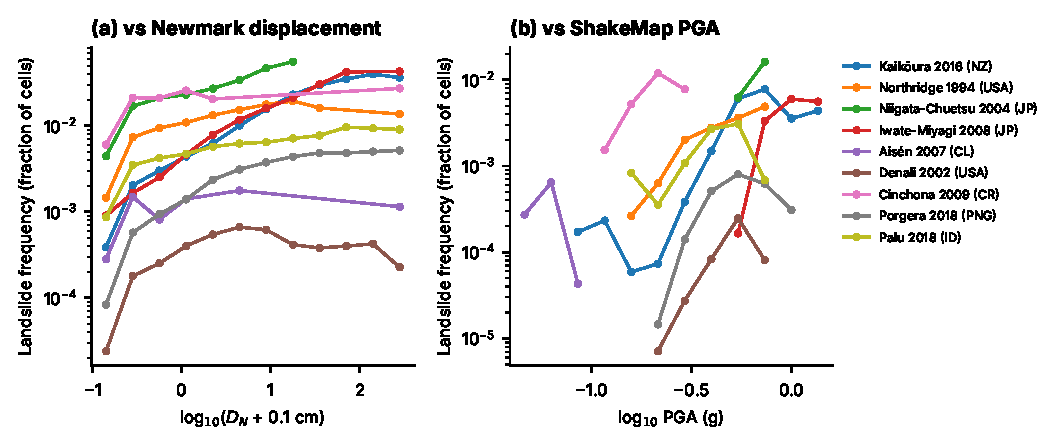
\includegraphics[width=\textwidth]{fig_response_curves.pdf}
\caption{Empirical landslide frequency (weighted fraction of 30~m cells containing a landslide) as a function of (a) Newmark displacement computed with uniform strength parameters and (b) ShakeMap PGA, for the nine earthquakes. Bins with fewer than five landslides are omitted. The curves have similar increasing shapes but are offset vertically by up to two orders of magnitude, which motivates the latent event offsets of HiPhyBoost.}\label{fig:response}
\end{figure*}

\section{Methods}\label{sec:methods}

\subsection{Physics feature: Newmark displacement}
Each cell is treated as an infinite slope with uniform, deliberately generic strength: effective friction angle $\phi'=32^\circ$, effective cohesion $c'=15$~kPa, unit weight $\gamma=20$~kN\,m$^{-3}$, slope-normal failure thickness $t=3$~m and dry conditions. These values follow the regional Newmark practice of \citet{jibson2000}, without event-specific geotechnical calibration. The static factor of safety and the critical acceleration (in units of $g$) are
\begin{equation}
FS = \frac{c'}{\gamma t \sin\alpha} + \frac{\tan\phi'}{\tan\alpha}, \qquad a_c = (FS-1)\sin\alpha ,
\end{equation}
where $\alpha$ is the slope angle. Permanent displacement $D_N$ (cm) is estimated from the ratio of $a_c$ to the ShakeMap PGA, $a_{\max}$, with the regression of \citet{jibson2007}:
\begin{equation}
\log_{10} D_N = 0.215 + \log_{10}\!\left[\left(1-\frac{a_c}{a_{\max}}\right)^{2.341}\left(\frac{a_c}{a_{\max}}\right)^{-1.438}\right], \qquad a_c<a_{\max},
\end{equation}
with $D_N=0$ where $a_c\ge a_{\max}$. Cells that are statically unstable ($FS<1$) are assigned a large displacement ($10^{2.5}$~cm). We use $\log_{10}(D_N+0.1)$ as a predictor. As a zero-parameter physics model we also map $D_N$ to failure probability with the Weibull curve calibrated on Northridge, $P=0.335\,[1-\exp(-0.048\,D_N^{1.565})]$ \citep{jibson2000}.

\subsection{Models}
Five models of increasing flexibility were compared, all using the same inputs.
\begin{description}
\item[Physics (Jibson 2000).] The Weibull curve above, with no fitting.
\item[Physics-logit.] Logistic regression on $\log_{10}(D_N+0.1)$ and slope. This keeps the Newmark mechanics but re-estimates the displacement--probability relation from the training events.
\item[Global LR.] Logistic regression on $\log_{10}$PGV, slope, their interaction and local relief. This mirrors the structure of the USGS global model \citep{nowickijessee2018} restricted to inputs available everywhere; lithology, land cover and wetness layers were not used.
\item[GBM.] Gradient-boosted trees \citep{friedman2001,chen2016} on the eleven predictors: eight terrain variables, $\log_{10}$PGA, $\log_{10}$PGV and $\log_{10}(D_N+0.1)$.
\item[PC-GBM.] The same learner and predictors, with monotonic constraints so that the predicted probability can only stay the same or increase with PGA, PGV, Newmark displacement, slope, maximum slope and local relief. The constraint encodes the physical expectation that stronger shaking or steeper, higher hillslopes cannot reduce the chance of failure, all else equal. It is a lightweight form of theory-guided learning \citep{karpatne2017}.
\end{description}
Both boosted models used the same fixed hyperparameters (400 trees, depth 4, learning rate 0.05, row and column subsampling 0.8, minimum child weight 5) and the \texttt{hist} algorithm of XGBoost 3.4. Hyperparameters were set a priori and never tuned on the held-out events, so the comparison does not favour either model.

\subsection{Sampling and weighting}
Each event domain contains between $4\times10^5$ and $2.7\times10^7$ cells. We kept all positive cells and a uniform random sample of $2.5\times10^5$ negative cells per event. Each negative was weighted by the inverse of its sampling fraction, so every weighted statistic refers to the full domain at its natural prevalence. During training, weights were also rescaled so that every training event has the same total weight. Without this, Kaik\={o}ura and Porgera would dominate the model; with it, each event counts as one independent realisation of coseismic landsliding.

\subsection{Experiment 1: leave-one-event-out transfer}
For each target event, the models were trained on the other eight events and evaluated on all cells of the target. As a local reference, which represents performance obtainable only after an inventory exists, PC-GBM was also evaluated within each event by five-fold spatial block cross-validation with 5~km blocks \citep{roberts2017}. Performance is reported on two axes. \emph{Discrimination} is measured with the area under the ROC curve (AUC) and the average precision divided by prevalence (AP lift, the factor by which the model concentrates landslides over random guessing). \emph{Calibration} is measured with the expected-to-observed ratio of landslide cells ($E/O=\sum_i w_i p_i / \sum_i w_i y_i$), the calibration slope and intercept from a logistic regression of outcomes on the predicted log-odds \citep{steyerberg2004,vancalster2019}, and the Brier skill score (BSS) relative to a climatological forecast that already knows the true prevalence \citep{brier1950}. Because BSS is referenced to the true prevalence, a transferred model must both rank and calibrate well to score above zero. Uncertainty in the AUC differences between models was estimated with a spatial block bootstrap (200 resamples of 5~km blocks).

\subsection{Experiment 2: few-shot recalibration}
In practice, emergency mapping delivers complete landslide maps for a few image tiles within days \citep{williams2018,handwerger2022}, long before an event-wide inventory exists. We simulated this by drawing $k\in\{1,2,5,10,20,40\}$ random $3\times3$~km tiles that contain at least one landslide, as an analyst would target visibly affected terrain. All cells in those tiles were labelled, and evaluation used the remaining cells of the event. Three updating strategies were applied to the transferred PC-GBM \citep{janssen2008}: (i) intercept-only recalibration, which shifts the log-odds by a constant $a$ chosen so that predicted and observed landslide counts agree in the mapped tiles; (ii) logistic (Platt) recalibration, which re-estimates intercept and slope; and (iii) for comparison, a new PC-GBM trained only on the mapped tiles. Each $(k,\text{event})$ combination was repeated 30 times with different random tiles.

\subsection{Experiment 3: attribution stability and physical consistency}
To test whether models learn the same controls in different earthquakes, we trained event-specific GBM and PC-GBM models and computed exact TreeSHAP values \citep{lundberg2020} for $2\times10^4$ cells per event. Stability was measured by the mean pairwise Spearman correlation between events of the mean absolute SHAP values of the eleven predictors, and by Kendall's coefficient of concordance $W$. Physical consistency of the transferred models was tested directly. For each held-out cell, PGA and PGV were increased by 10\%, Newmark displacement was recomputed, and we recorded the fraction of cells whose predicted probability \emph{decreased}. Such a decrease is a physically implausible response.

All processing used open data and open-source software (Python, GDAL/rasterio, XGBoost, scikit-learn). The code that reproduces every number and figure is available in the accompanying repository.

\section{Results}\label{sec:results}
We first report the baseline models (Experiment~1), whose behaviour motivates the proposed algorithm, and then HiPhyBoost (Sections~\ref{sec:res_hiphy}--\ref{sec:res_fewshot}).

\begin{table}[t]\centering\small
\caption{The nine Pacific Rim earthquakes, their study domains and landslide statistics on the 30~m grid. Prevalence is the percentage of domain cells that contain a landslide point. PGA values are from the USGS ShakeMap used as model input.}\label{tab:events}
\resizebox{\textwidth}{!}{\begin{tabular}{lrrrrrrr}\toprule
Event & M\textsubscript{w} & Domain (km$^2$) & Landslides & Positive cells & Prevalence (\%) & PGA$_{\max}$ (g) & mean PGA at landslides (g)\\\midrule
Kaik\={o}ura 2016 (NZ) & 7.8 & 10\,832 & 29\,519 & 28\,474 & 0.237 & 1.61 & 0.64 \\
Northridge 1994 (USA) & 6.7 & 4\,377 & 11\,111 & 10\,925 & 0.225 & 0.87 & 0.48 \\
Niigata-Chuetsu 2004 (JP) & 6.6 & 410 & 4\,862 & 4\,860 & 1.067 & 0.82 & 0.70 \\
Iwate-Miyagi 2008 (JP) & 6.9 & 777 & 4\,164 & 4\,093 & 0.474 & 1.20 & 0.96 \\
Ais\'{e}n 2007 (CL) & 6.2 & 1\,247 & 517 & 512 & 0.037 & 0.12 & 0.06 \\
Denali 2002 (USA) & 7.9 & 15\,748 & 1\,579 & 1\,579 & 0.009 & 0.74 & 0.49 \\
Cinchona 2009 (CR) & 6.1 & 637 & 4\,826 & 4\,743 & 0.670 & 0.27 & 0.19 \\
Porgera 2018 (PNG) & 7.5 & 24\,306 & 10\,469 & 10\,455 & 0.039 & 1.05 & 0.53 \\
Palu 2018 (ID) & 7.5 & 3\,665 & 7\,063 & 7\,007 & 0.172 & 0.88 & 0.43 \\
\bottomrule\end{tabular}}\end{table}


\begin{figure*}[t]\centering
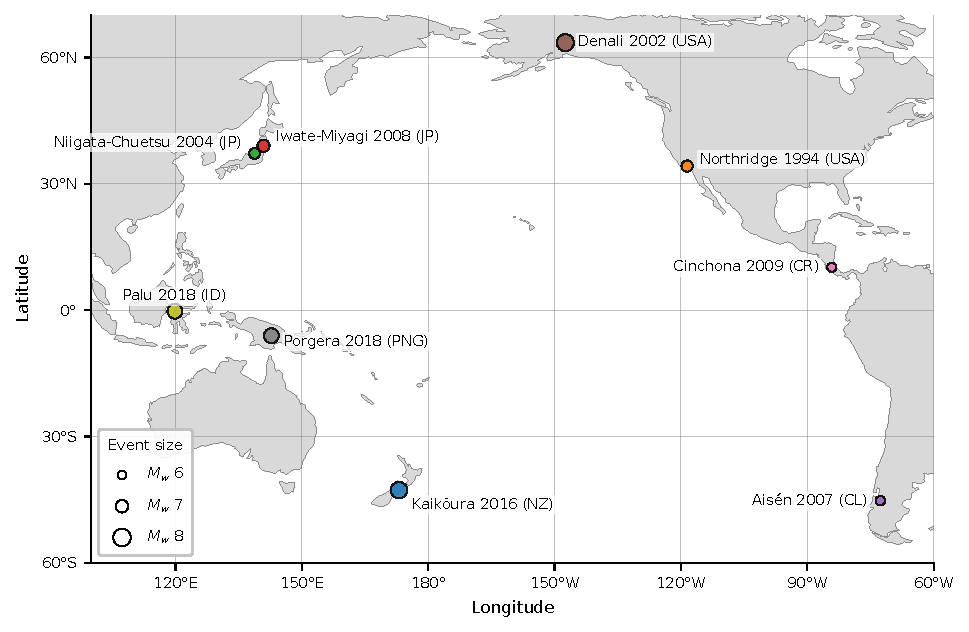
\includegraphics[width=\textwidth]{fig1_events.pdf}
\caption{The nine Pacific Rim earthquakes analysed. Marker size scales with moment magnitude.}\label{fig:events}
\end{figure*}

\begin{figure*}[t]\centering
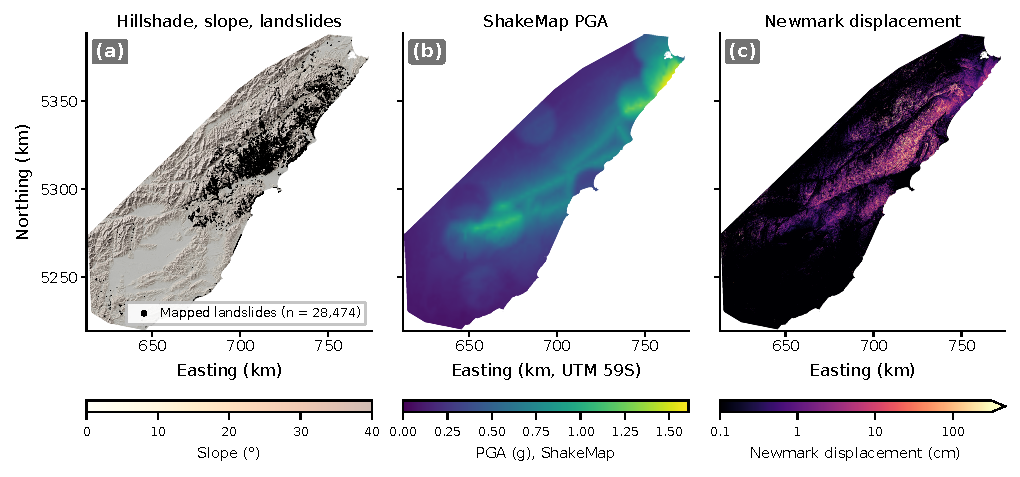
\includegraphics[width=\textwidth]{fig2_kaikoura_inputs.pdf}
\caption{Model inputs for the 2016 Kaik\={o}ura earthquake on the 30~m analysis grid (UTM zone 59S). (a) Copernicus GLO-30 hillshade and slope with the 28\,474 landslide cells of the GNS Science inventory; (b) USGS ShakeMap peak ground acceleration; (c) Newmark displacement computed with uniform generic strength parameters.}\label{fig:kaikoura_inputs}
\end{figure*}

\subsection{Transfer of discrimination}
Table~\ref{tab:loeo} and Figure~\ref{fig:loeo} summarise Experiment~1. Every transferred model discriminates landslide from non-landslide cells better than chance in most events. The ordering of the models, however, depends on the target event. The physics-constrained PC-GBM has the highest median AUC across held-out events (0.805), followed by the unconstrained GBM (0.790), the two Newmark models (0.763--0.764) and the global-style logistic regression (0.750). Its advantage lies in robustness more than in average skill. By median AP lift, the unconstrained GBM and the global LR (3.9 each) slightly exceed PC-GBM (3.4). PC-GBM has the highest worst-case AUC of all models (0.730, Palu), whereas the worst cases of GBM (0.639) and the physics curve (0.559) fall in the low-shaking Ays\'en and Cinchona events. The global LR fails completely there, with AUC 0.247 and 0.397: its ranking is inverted.

The spatial block bootstrap gives the paired differences. PC-GBM is significantly better than the global LR in seven events (95\% intervals exclude zero; median gain 0.06 AUC at Kaik\={o}ura and 0.37--0.51 at Cinchona and Ays\'en), equivalent at Palu and worse at Denali ($-0.024$). Compared with the unconstrained GBM, PC-GBM is significantly better at Northridge ($+0.025$), Niigata ($+0.014$), Iwate ($+0.037$) and Ays\'en ($+0.119$), equivalent at Kaik\={o}ura, Cinchona and Porgera, and worse at Denali ($-0.045$) and Palu ($-0.059$). The monotonic constraints therefore cost little where the unconstrained learner already transfers well, and they prevent large failures where it does not.

Transfer does not reach the skill of a model fitted to the event itself. The local PC-GBM, evaluated with spatial-block cross-validation, has median AUC 0.838 and median AP lift 5.7, compared with 0.805 and 3.4 for the transferred PC-GBM. The gap ranges from almost nothing at Iwate (0.833 vs 0.834) to 0.08 at Northridge. For Kaik\={o}ura, PC-GBM trained only on the eight other Pacific Rim events reaches AUC 0.887 and concentrates landslides 9.2 times more than random (AP lift), against 0.934 and 16.8 for the local model.

\begin{table*}[t]\centering\small
\caption{Leave-one-event-out transfer. ROC AUC on each held-out event for the five models trained on the other eight events (best transferred model in bold), the AUC of a local PC-GBM evaluated by 5~km spatial-block cross-validation within the event, and calibration of the transferred PC-GBM: the expected-to-observed ratio of landslide cells ($E/O$, ideal 1) and the calibration slope (ideal 1).}\label{tab:loeo}
\resizebox{\textwidth}{!}{\begin{tabular}{lrrrrrrrr}\toprule
 & \multicolumn{5}{c}{Transferred (LOEO) AUC} & Local AUC & \multicolumn{2}{c}{PC-GBM calibration}\\
\cmidrule(lr){2-6}\cmidrule(lr){8-9}
Event & Physics & Phys.-logit & Global LR & GBM & PC-GBM & PC-GBM & $E/O$ & slope\\\midrule
Kaik\={o}ura 2016 (NZ) & 0.883 & 0.861 & 0.826 & \textbf{0.894} & 0.887 & 0.934 & 1.50 & 1.07\\
Northridge 1994 (USA) & 0.715 & 0.756 & 0.723 & 0.788 & \textbf{0.814} & 0.893 & 0.94 & 0.96\\
Niigata-Chuetsu 2004 (JP) & 0.763 & 0.767 & 0.750 & 0.774 & \textbf{0.788} & 0.809 & 0.23 & 0.88\\
Iwate-Miyagi 2008 (JP) & 0.777 & 0.764 & 0.750 & 0.796 & \textbf{0.833} & 0.834 & 2.58 & 1.20\\
Ais\'{e}n 2007 (CL) & 0.609 & 0.739 & 0.247 & 0.639 & \textbf{0.760} & 0.826 & 1.11 & 0.99\\
Denali 2002 (USA) & 0.831 & 0.845 & 0.830 & \textbf{0.850} & 0.805 & 0.883 & 23.40 & 1.53\\
Cinchona 2009 (CR) & 0.559 & 0.734 & 0.397 & \textbf{0.780} & 0.774 & 0.812 & 0.02 & 0.82\\
Porgera 2018 (PNG) & 0.885 & \textbf{0.892} & 0.847 & 0.876 & 0.872 & 0.934 & 8.84 & 1.40\\
Palu 2018 (ID) & 0.742 & 0.762 & 0.733 & \textbf{0.790} & 0.730 & 0.838 & 1.89 & 1.08\\
\midrule Median & 0.763 & 0.764 & 0.750 & 0.790 & 0.805 & 0.838 & 1.50 & 1.07\\
Minimum & 0.559 & 0.734 & 0.247 & 0.639 & 0.730 & 0.809 & & \\
\bottomrule\end{tabular}}\end{table*}


\begin{figure*}[t]\centering
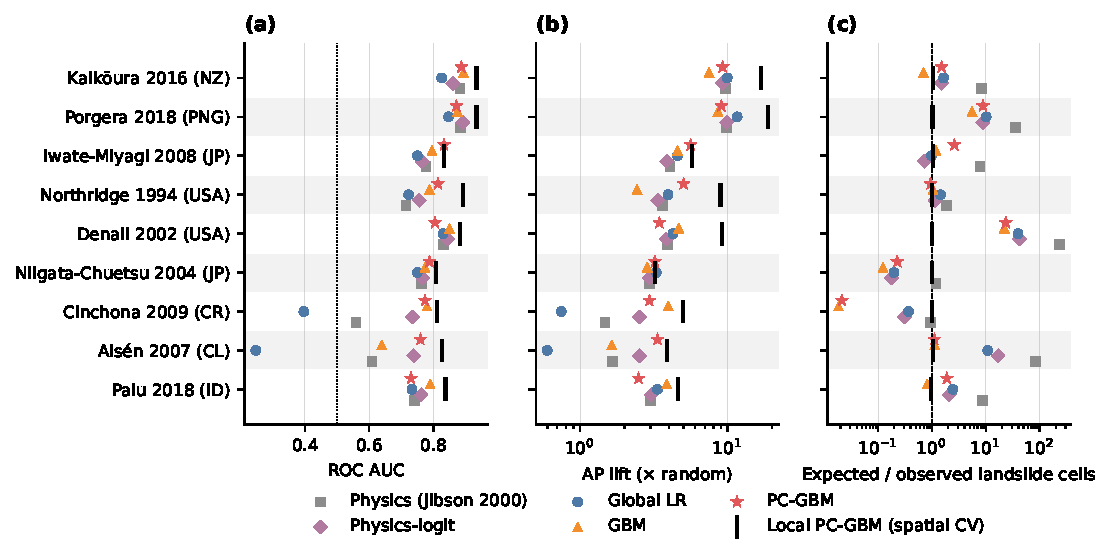
\includegraphics[width=\textwidth]{fig3_loeo.pdf}
\caption{Leave-one-event-out transfer of five models to each of the nine earthquakes. (a) ROC AUC; (b) average precision divided by prevalence; (c) ratio of expected to observed landslide cells (log scale, ideal 1). Vertical bars show a PC-GBM trained and tested within the event by spatial-block cross-validation.}\label{fig:loeo}
\end{figure*}

\subsection{Why the global logistic model inverts}
The inversion of the global LR at Ays\'en and Cinchona follows from its functional form under covariate shift. Fitted on the other events, it combines a negative slope main effect with a positive slope--PGV interaction. The effect of slope on the log-odds therefore turns negative below a PGV of about 4--9~cm\,s$^{-1}$, which is where most cells of these two low-shaking ShakeMaps lie (Supplementary Section~S3). Tree ensembles extrapolate as constants beyond the training range and do not invert.

\subsection{Transfer of calibration}
Transferred models rank hillslopes reasonably well, but their probabilities are badly calibrated (Figure~\ref{fig:loeo}c; Supplementary Figure~S2). For PC-GBM the expected-to-observed ratio of landslide cells ranges from 0.02 at Cinchona (50 times too few landslides predicted) to 23 at Denali (23 times too many), and lies within a factor of two of the truth in only four of the nine events (Kaik\={o}ura, Northridge, Ays\'en and Palu). The uncalibrated Newmark--Weibull curve of \citet{jibson2000} overpredicts in eight events, by a factor of 8 at Kaik\={o}ura and up to 228 at Denali. Its calibration slopes of 0.1--0.4 show that its probabilities are also far too spread out. In contrast, the calibration slopes of the transferred PC-GBM are close to one (median 1.07, range 0.82--1.53). The miscalibration of the learned models is therefore mostly a \emph{shift} in the overall level of landslide occurrence, not an error in the shape of the response. This is the behaviour expected when the event-level base rate differs between source and target, and it can be corrected by recalibrating the intercept, which motivates Experiment~2.

Brier skill scores are close to zero for all fitted models, including the local models (local PC-GBM: 0.000--0.017; transferred PC-GBM: $-0.20$ to $+0.01$), and strongly negative for the uncalibrated physics curve. With landslide prevalence of 0.01--1\%, the squared-error gain from ranking is small compared with the cost of any error in the base rate. BSS is therefore a poor guide to the usefulness of a coseismic model, and we use $E/O$ and the calibration slope as the main calibration diagnostics.



\subsection{HiPhyBoost: transfer of discrimination}\label{sec:res_hiphy}
Estimating event offsets jointly with the shared response improves transfer in most events. In the same leave-one-event-out design, HiPhyBoost reaches a median AUC of 0.833 and a median AP lift of 4.1, compared with 0.805 and 3.4 for PC-GBM and 0.790 and 3.9 for the unconstrained GBM (Table~\ref{tab:hiphy}). The ablation with offsets fixed at zero keeps the Newmark anchor, the constraints and the larger number of trees (700 instead of 400) but removes the offsets. It reaches 0.810, practically equal to PC-GBM (mean difference $+0.001$). The gain is therefore due to the offsets, not to the physics anchor or the larger tree budget. The spatial block bootstrap shows that HiPhyBoost is significantly better than PC-GBM at Kaik\={o}ura ($+0.030$; 95\% interval $0.021$--$0.038$), Northridge ($+0.019$), Denali ($+0.042$), Porgera ($+0.044$) and Palu ($+0.049$). It is equivalent at Niigata and Iwate, and slightly worse at Ays\'en ($-0.025$) and Cinchona ($-0.013$), the two events with very weak ShakeMap shaking. These bootstrap intervals describe uncertainty within each event. Treating the nine events as the units of replication, HiPhyBoost is better than PC-GBM in six of nine events (mean $\Delta$AUC $+0.016$, median $+0.019$), but the difference is not significant with nine events (Wilcoxon signed-rank $p=0.16$; against the unconstrained GBM $p=0.07$; against the global LR $p=0.004$). The improvement is therefore consistent but modest, and it should be confirmed with further inventories. For Kaik\={o}ura, the model trained only on the eight other Pacific Rim earthquakes reaches AUC 0.917 and concentrates landslides 12.7 times more than random. This is close to the local model fitted to the Kaik\={o}ura inventory itself (AUC 0.934, AP lift 16.8), and the predicted landslide density at 2~km resolution agrees with the GNS inventory with Spearman $\rho=0.61$ (Figure~\ref{fig:kaikoura}). Similar rank agreement at 2~km is obtained for Northridge, Iwate, Porgera and Palu ($\rho=0.51$--$0.64$; Figure~\ref{fig:maps}).

Why does modelling the level improve the ranking? In a pooled model, an event with a high base rate, such as Cinchona or Niigata, pulls the shared response towards predictors that happen to separate that event from the others, for example low PGV or particular terrain textures. These predictors then act as proxies for ``being in a landslide-prone earthquake'' rather than for ``being a susceptible hillslope''. Once each event has its own offset, between-event differences are absorbed by $b_e$, and the trees are fitted to within-event contrasts, which are the contrasts that matter when ranking hillslopes in a new earthquake. The two events where HiPhyBoost loses are those where within-event shaking contrasts are weakest (Supplementary Figure~S1): ranking there depends almost entirely on terrain, and pooling information on the base rate from the other events helps PC-GBM slightly.

\begin{table*}[t]\centering\small
\caption{Leave-one-event-out transfer of HiPhyBoost. AUC of the transferred PC-GBM, of HiPhyBoost without event offsets (ablation) and of the full HiPhyBoost ($^{*}$: 95\% block-bootstrap interval of the difference from PC-GBM excludes zero); AP lift; ratio of predicted to observed landslide cells for the HiPhyBoost point forecast ($E/O$); 90\% zero-shot predictive interval of $E/O$ and whether it contains 1.}\label{tab:hiphy}
\resizebox{\textwidth}{!}{\begin{tabular}{lrrrrrrlc}\toprule
 & \multicolumn{3}{c}{AUC} & \multicolumn{2}{c}{AP lift} & & \multicolumn{2}{c}{Zero-shot 90\% interval}\\\cmidrule(lr){2-4}\cmidrule(lr){5-6}\cmidrule(lr){8-9}
Event & PC-GBM & No offsets & HiPhyBoost & PC-GBM & HiPhyBoost & $E/O$ & $E/O$ interval & covers\\\midrule
Kaik\={o}ura 2016 (NZ) & 0.887 & 0.888 & \textbf{0.917}$^{*}$ & 9.2 & 12.7 & 1.06 & [0.060, 15.9] & yes\\
Northridge 1994 (USA) & 0.814 & 0.815 & \textbf{0.833}$^{*}$ & 5.0 & 6.1 & 0.46 & [0.026, 7.5] & yes\\
Niigata-Chuetsu 2004 (JP) & 0.788 & 0.794 & \textbf{0.784} & 3.2 & 3.0 & 0.13 & [0.008, 1.9] & yes\\
Iwate-Miyagi 2008 (JP) & 0.833 & 0.835 & \textbf{0.834} & 5.6 & 5.4 & 1.12 & [0.052, 19.2] & yes\\
Ais\'{e}n 2007 (CL) & 0.760 & 0.747 & \textbf{0.734}$^{*}$ & 3.3 & 2.8 & 0.15 & [0.008, 3.0] & yes\\
Denali 2002 (USA) & 0.805 & 0.810 & \textbf{0.848}$^{*}$ & 3.4 & 4.1 & 33.68 & [4.114, 241.7] & no\\
Cinchona 2009 (CR) & 0.774 & 0.776 & \textbf{0.760}$^{*}$ & 2.9 & 2.8 & 0.02 & [0.002, 0.2] & no\\
Porgera 2018 (PNG) & 0.872 & 0.877 & \textbf{0.916}$^{*}$ & 9.1 & 13.0 & 6.12 & [0.396, 79.7] & yes\\
Palu 2018 (ID) & 0.730 & 0.734 & \textbf{0.780}$^{*}$ & 2.5 & 3.7 & 1.24 & [0.065, 20.9] & yes\\
\midrule Median & 0.805 & 0.810 & 0.833 & 3.4 & 4.1 & 1.06 & & 7/9\\
\bottomrule\end{tabular}}\end{table*}


\subsection{Event offsets as a geoscientific quantity}\label{sec:res_offsets}
Fitted on all nine events, the offsets span 5.7 log-odds units, from $b=-3.15$ at Denali to $+2.59$ at Cinchona ($\tau=1.69$; Figure~\ref{fig:offsets}a). In other words, with terrain and computed Newmark displacement held equal, the odds of a landslide cell were about 300 times higher at Cinchona than at Denali. Offsets are strongly positive for Cinchona ($+2.6$) and Niigata-Chuetsu ($+1.7$) and moderately positive for Northridge ($+0.7$). They are close to zero for Ays\'en, Iwate, Kaik\={o}ura and Palu, and strongly negative for Porgera ($-1.6$) and Denali ($-3.2$). The offsets are stable across the leave-one-event-out folds (standard deviation of each event's offset across the eight folds in which it is a training event: 0.18--0.33 log-odds units, small compared with the 5.7-unit spread between events), so they are a robust property of the data, not an artefact of a particular fit. Their interpretation is discussed in Section~\ref{sec:disc}.

\subsection{Zero-shot forecasts of the landslide total}
Without any mapped landslide, the transferred point forecast of HiPhyBoost (the offset set to the prior median; the Bayesian predictive mean is a poor point forecast because the lognormal-like uncertainty of the total makes it overpredict, median $E/O=3.7$) is within a factor of two of the observed number of landslide cells in three events (Iwate, Kaik\={o}ura, Palu), compared with four for PC-GBM. Neither model can predict the base rate of an unseen earthquake, because the offsets are not explained by the inputs. The value of the Bayesian formulation is that it makes this ignorance explicit. The 90\% predictive interval of the landslide total spans a factor of 60--390, and it contains the observed total in seven of nine events (Figure~\ref{fig:offsets}b). Such wide intervals are only weakly informative, but they are honest. Replacing the normal prior by a Student-$t$ predictive that accounts for estimating $\mu$ and $\tau$ from eight events widens them further (median factor 850) without changing the coverage. The two misses are Cinchona, observed above the interval, and Denali, observed below it, the events with the most extreme offsets. PC-GBM gives a single number in every case and no indication that, for example, its forecast for Cinchona is 50 times too low. For emergency planning, an interval spanning two orders of magnitude at least shows how uncertain the forecast is, which a point estimate wrong by the same amount does not. It also shows directly how much the forecast stands to gain from early mapping, which Experiment~2 quantifies.

\begin{figure*}[t]\centering
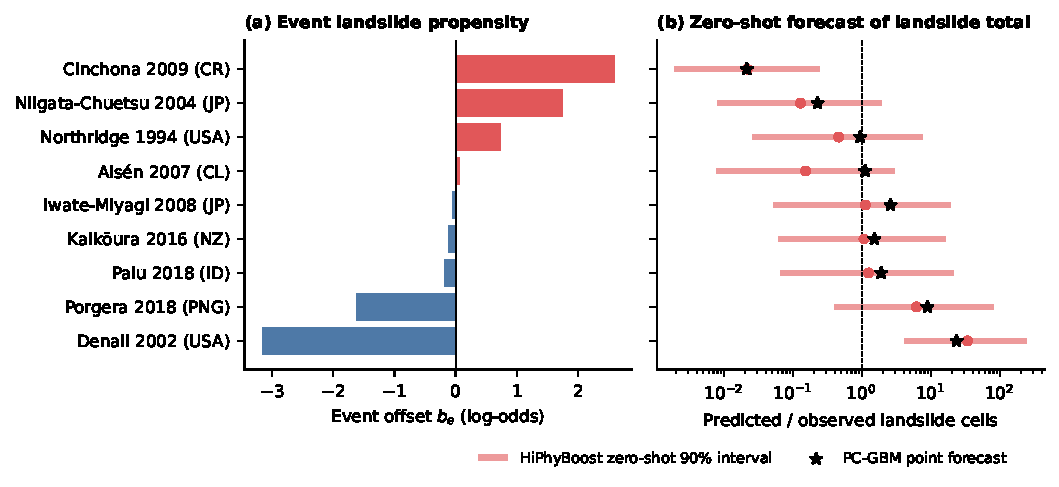
\includegraphics[width=\textwidth]{fig8_offsets.pdf}
\caption{(a) Event offsets $b_e$ of HiPhyBoost fitted on all nine earthquakes: the landslide propensity of each event relative to the population, with terrain and Newmark displacement held equal. (b) Zero-shot forecasts of the total number of landslide cells for each held-out event: HiPhyBoost 90\% predictive interval (bar) and median (dot), and the PC-GBM point forecast (star), all relative to the observed total (dashed line).}\label{fig:offsets}
\end{figure*}

\begin{figure*}[t]\centering
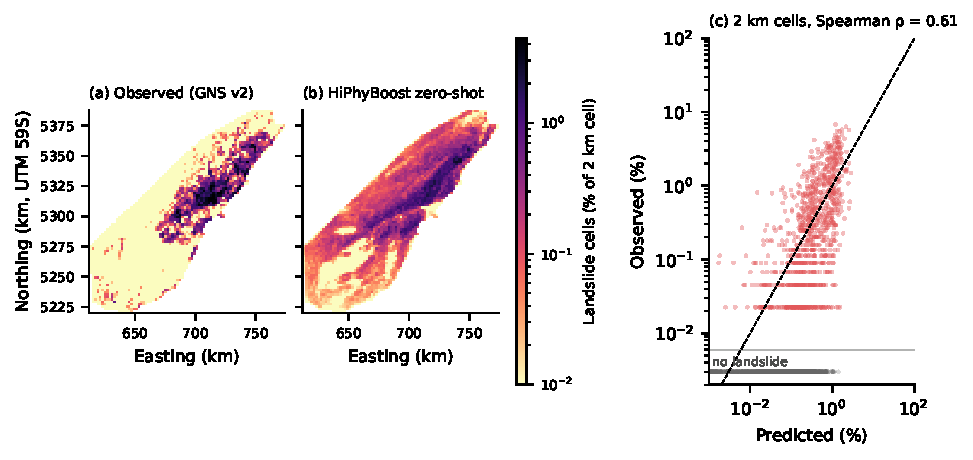
\includegraphics[width=\textwidth]{fig7_kaikoura_transfer.pdf}
\caption{Zero-shot transfer to the 2016 Kaik\={o}ura earthquake. (a) Observed percentage of 30~m cells containing a landslide source in 2~km cells (GNS Science inventory v2); (b) HiPhyBoost forecast trained only on the eight other Pacific Rim earthquakes (offset at the prior median); (c) predicted against observed density for 2~km cells; cells without any mapped landslide are shown in the bottom strip.}\label{fig:kaikoura}
\end{figure*}

\begin{figure*}[t]\centering
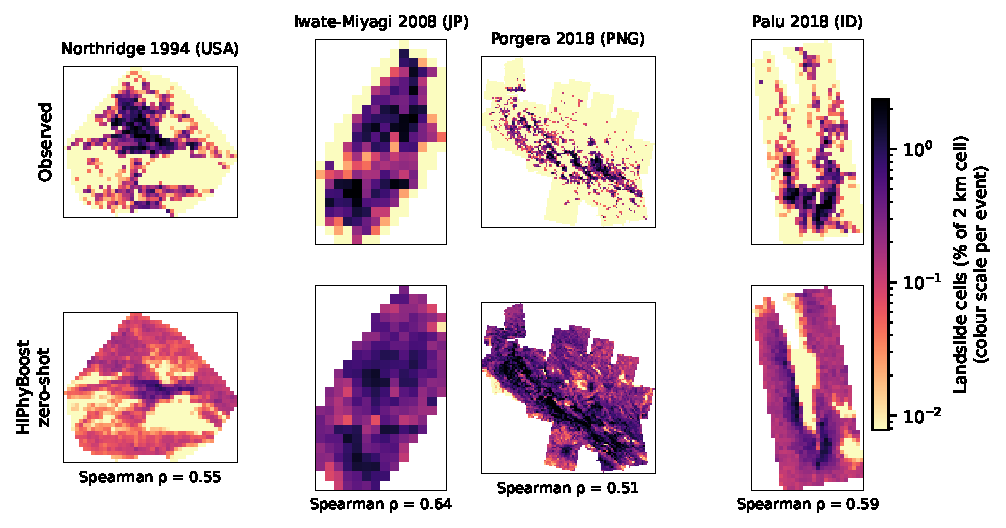
\includegraphics[width=\textwidth]{fig10_maps_multi.pdf}
\caption{Observed (top) and HiPhyBoost zero-shot (bottom) landslide density at 2~km resolution for four further held-out events. Each column uses its own colour scale; $\rho$ is the Spearman correlation between predicted and observed density over 2~km cells.}\label{fig:maps}
\end{figure*}

\subsection{Few-shot updating from rapid mapping}\label{sec:res_fewshot}
Table~\ref{tab:fewshot} and Figure~\ref{fig:fewshot} summarise Experiment~2. Because updating changes only the offset, it leaves the ranking of cells unchanged, and HiPhyBoost keeps its advantage in discrimination over PC-GBM at every $k$ (median AUC 0.834--0.841 against 0.805--0.816). The differences between methods lie in the predicted landslide total and in its uncertainty.

\emph{Point accuracy.} After one mapped tile, recalibrated PC-GBM still mispredicts the landslide total in the unmapped area by a median factor of $2^{1.31}=2.5$, and the cell-level HiPhyBoost posterior by a factor of 2.2. The full HiPhyBoost quasi-posterior reduces this to a factor of 1.6 ($|\log_2 E/O|=0.68$), because a single tile no longer overrides the prior learned from eight past earthquakes. With five to ten tiles the error falls to a factor of about 1.4 (0.48--0.53), against 1.6 for recalibrated PC-GBM. All methods lose some accuracy at $k=40$, probably because the remaining unmapped area is then dominated by sparsely affected terrain, whose landslide density an offset fitted to the most affected tiles overstates.

\emph{Uncertainty.} The cell-level Bayesian posterior is far too confident. Its 90\% intervals contain the observed total in only 4--26\% of draws, because it treats the several thousand cells of a mapped tile as independent evidence. The measured dispersion of tile-level counts shows how wrong this is. Evaluated with each event's own fitted offset, $\phi$ ranges from 7 (Denali) to 193 (Cinchona). The values actually used in the update, the medians over the eight training events of each fold, are 47--68. A mapped tile therefore carries roughly one fiftieth of the information that the independence assumption gives it (Figure~\ref{fig:posterior}). The quasi-posterior raises coverage to 0.72--0.76 for $k\le 10$ and 0.70 at $k=20$. At the same time the interval for the remaining landslide total narrows from a factor of 59 after one tile to a factor of 6.5 after five and 3.7 after ten. Coverage stays below the nominal 90\% because a single dispersion factor cannot represent events as different as Denali and Cinchona, and it declines at $k=40$, when chosen tiles begin to share landslide clusters.

\emph{Selection.} Within the quasi-likelihood formulation the selection term has almost no effect (coverage 0.54 against 0.51 at $k=40$; otherwise identical). Once the likelihood is divided by $\phi$, the selection penalty is down-weighted by the same factor, and the bias it corrects is small compared with the dispersion. The selection term matters a great deal in the alternative Gaussian tile-random-effect formulation: there it raises coverage at $k=10$ from 0.20 to 0.74 and reduces the point error by about 40\%. That formulation, however, has a large point bias for the landslide total (factors of 2.5--4.4 after one to ten tiles). A Gaussian random effect cannot represent the real distribution of landslides over tiles, in which most tiles hold none and a few hold hundreds. We therefore recommend the quasi-posterior as the default form of component~(iii). The selection term costs nothing and protects against stronger targeting than our uniform-among-affected-tiles protocol simulates.

\begin{table*}[t]\centering\small
\caption{Few-shot updating from $k$ rapidly mapped $3\times3$~km tiles (Experiment~2; identical tile draws for all methods, 30 repetitions per event and $k$). $|\log_2 E/O|$: absolute log$_2$ ratio of predicted to observed landslide cells in the unmapped area (median over events of per-event medians; 1 = a factor of two). Coverage: share of draws in which the 90\% predictive interval contained the observed total (mean over events; nominal 0.90). Width: ratio of the upper to the lower interval bound (median).}\label{tab:fewshot}
\resizebox{\textwidth}{!}{\begin{tabular}{lrrrrrrrrrr}\toprule
 & \multicolumn{4}{c}{$|\log_2 E/O|$} & \multicolumn{4}{c}{90\% coverage} & \multicolumn{2}{c}{Width}\\\cmidrule(lr){2-5}\cmidrule(lr){6-9}\cmidrule(lr){10-11}
Method & $k$=1 & 5 & 10 & 40 & 1 & 5 & 10 & 40 & $k$=1 & 10\\\midrule
PC-GBM, intercept recalibration & 1.31 & 0.64 & 0.71 & 0.64 & -- & -- & -- & -- & -- & --\\
PC-GBM, Platt recalibration & 1.37 & 0.69 & 0.68 & 0.67 & -- & -- & -- & -- & -- & --\\
HiPhyBoost, ML offset & 1.17 & 0.62 & 0.52 & 0.60 & -- & -- & -- & -- & -- & --\\
HiPhyBoost, cell-level Bayes & 1.14 & 0.64 & 0.52 & 0.60 & 0.26 & 0.19 & 0.16 & 0.04 & 2.3 & 1.2\\
\quad + selection term & 1.14 & 0.61 & 0.52 & 0.59 & 0.26 & 0.19 & 0.17 & 0.04 & 2.3 & 1.2\\
HiPhyBoost, tile random effect & 2.57 & 2.26 & 2.27 & 2.38 & 0.79 & 0.44 & 0.20 & 0.00 & 70 & 6.0\\
\quad + selection term & 2.15 & 1.35 & 1.37 & 1.47 & 0.82 & 0.85 & 0.74 & 0.19 & 114 & 9.2\\
HiPhyBoost, quasi-Bayes & 0.66 & 0.52 & 0.48 & 0.58 & 0.73 & 0.74 & 0.72 & 0.51 & 58 & 3.7\\
\quad + selection term (full HiPhyBoost) & 0.68 & 0.53 & 0.48 & 0.58 & 0.73 & 0.74 & 0.72 & 0.54 & 59 & 3.7\\
\bottomrule\end{tabular}}\end{table*}


\begin{figure*}[t]\centering
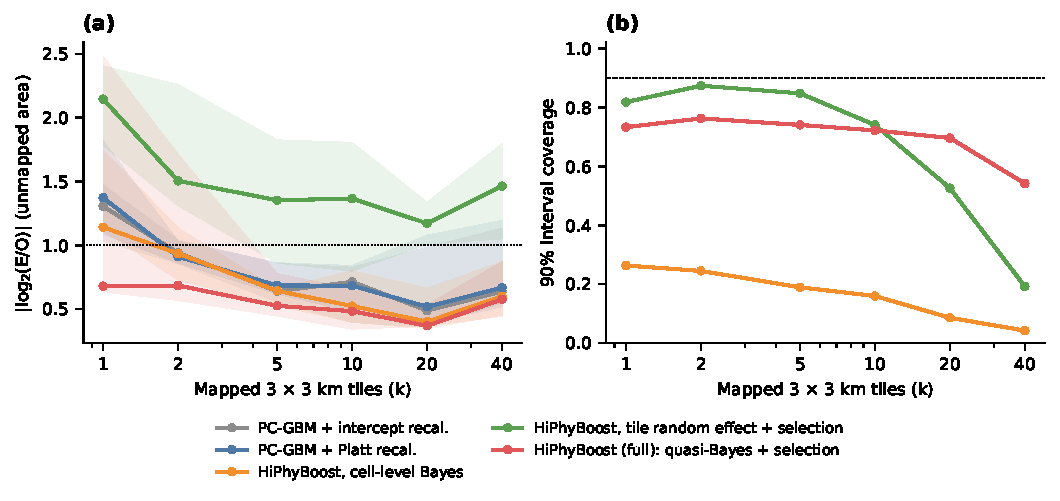
\includegraphics[width=\textwidth]{fig5_fewshot.pdf}
\caption{Few-shot updating from $k$ rapidly mapped $3\times3$~km tiles, evaluated on the unmapped part of each held-out event. (a) Absolute $\log_2$ ratio of predicted to observed landslide cells (1 = a factor of two); (b) coverage of the 90\% predictive interval of the landslide total (dashed: nominal). Lines: median (a) or mean (b) over events; shading: interquartile range over events. At $k=40$, Niigata-Chuetsu is excluded because it has fewer than 80 tiles.}\label{fig:fewshot}
\end{figure*}

\begin{figure*}[t]\centering
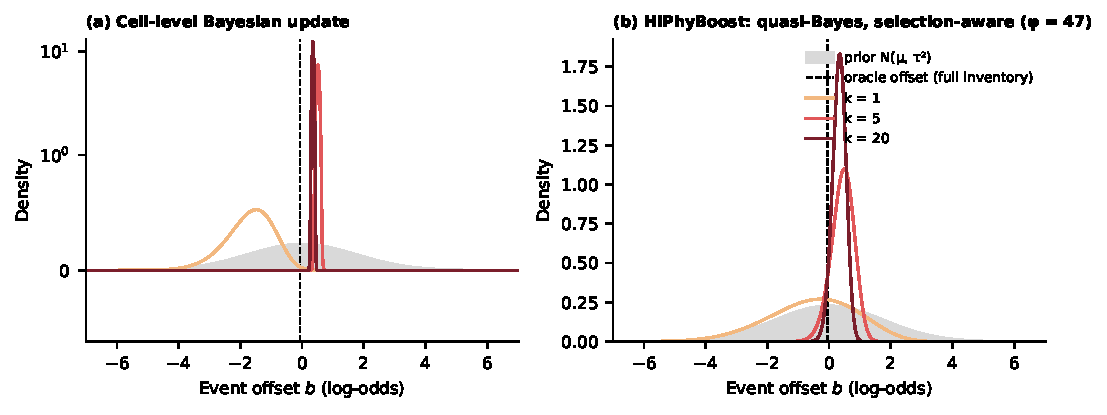
\includegraphics[width=\textwidth]{fig9_posterior_kaikoura.pdf}
\caption{Posterior of the Kaik\={o}ura event offset after mapping $k=1$, 5 and 20 randomly chosen landslide-bearing tiles, using HiPhyBoost scores transferred from the eight other earthquakes. (a) A cell-level Bayesian update (note the logarithmic density axis) concentrates on a wrong value after a few tiles. (b) The HiPhyBoost quasi-posterior with dispersion factor $\phi$ narrows gradually and stays consistent with the offset implied by the complete inventory (dashed).}\label{fig:posterior}
\end{figure*}

\subsection{Attribution stability and physical consistency}\label{sec:res_shap}
Figure~\ref{fig:shap} summarises Experiment~3; its interpretation is given in Section~\ref{sec:disc}. Event-specific models agree only moderately on predictor importance (mean pairwise Spearman correlation 0.42 for GBM and 0.31 for PC-GBM). This is well above the agreement expected between random importance rankings (95th percentile 0.09), but far from consistent. Grouping the correlated predictors gives a more stable picture: for GBM, terrain variables account for 44--73\% of the mean absolute attribution, ground motion (PGA, PGV) for 24--41\% and Newmark displacement for 0.5--28\% in individual events. Maximum local slope, PGA, Newmark displacement and PGV are the most important predictors on average. Increasing PGA and PGV by 10\% lowered the predicted probability in a mean of 26\% of held-out cells for the transferred GBM and 43\% for the global LR, and in none for the constrained models.

\begin{figure*}[t]\centering
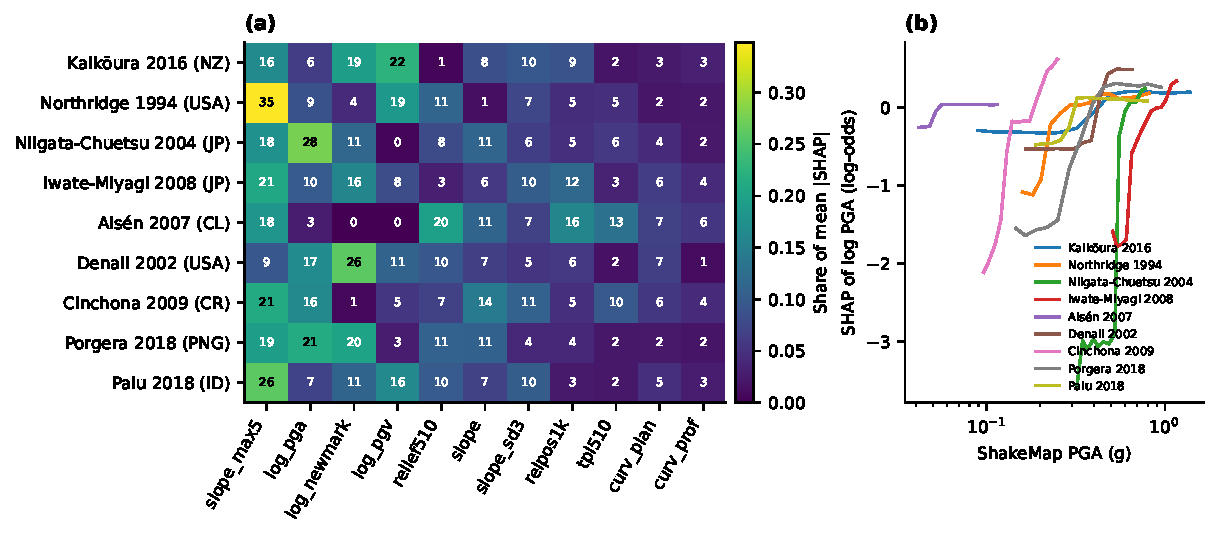
\includegraphics[width=\textwidth]{fig6_shap.pdf}
\caption{TreeSHAP attributions of event-specific PC-GBM models. (a) Share of the mean absolute SHAP value of each predictor (\%) for each event; predictors ordered by mean importance. (b) SHAP dependence of $\log_{10}$PGA (binned medians) for each event: the response is monotone in all events, but the PGA at which it rises differs by almost an order of magnitude.}\label{fig:shap}
\end{figure*}

\section{Discussion}\label{sec:disc}

\subsection{What transfers between earthquakes, and what does not}
Two signals are mixed in a coseismic landslide map: the \emph{relative} susceptibility of hillslopes to a given shaking field, and the \emph{absolute} level of landsliding in that event. Our results show that the first transfers reasonably well across very different Pacific Rim settings, and the second does not. Transferred models from all three learned families rank cells with AUC of about 0.73--0.89 in most events, and their calibration slopes near one show that the shape of the probability response is also approximately preserved. The base rate, by contrast, is mispredicted over a range of about three orders of magnitude, from $E/O=0.02$ at Cinchona to $E/O=23$ at Denali. Equal shaking and equal topography therefore produce very different numbers of landslides in different earthquakes. Some of this variation is genuine geoscience; some is a property of the inventories and ShakeMaps.

The events with the largest offsets have known, process-level explanations that our inputs do not include. At Denali the transferred models overpredict by a factor of more than 20. \citet{gorum2014denali} explicitly asked why this M\textsubscript{w}~7.9 earthquake triggered so few landslides, and \citet{jibson2004} used the sparse landsliding to infer the character of the strong shaking. Their explanations, discussed in those studies, involve rupture and site characteristics that a PGA and PGV field does not capture. At Niigata-Chuetsu ($E/O=0.23$) the earthquake struck weak Neogene sediments shortly after heavy typhoon rainfall \citep{sassa2005}. Antecedent pore pressure is outside our dry Newmark formulation and outside the static predictors. At Cinchona ($E/O=0.02$) the models predict almost no landslides because the ShakeMap Atlas gives a median PGA of only 0.19~g at the landslide cells and a maximum of 0.27~g in the domain. Yet thousands of slides, many of which became mudflows \citep{alvarado2009}, occurred on deeply weathered volcanic slopes. Either the ShakeMap underestimates near-source shaking for this shallow M\textsubscript{w}~6.1 event, or the volcanic soils fail at unusually low accelerations; most likely both contribute. At Porgera ($E/O=8.8$) the mapped domain is the largest of all events (24\,306~km$^2$), and dense tropical forest and persistent cloud may have limited the detectability of small slides. Mapping completeness thus probably adds to whatever physical difference exists \citep{tanyas2017,tanyas2022png}. These cases show that an event-level offset is itself a geoscientific quantity. It integrates antecedent wetness, material strength, shaking error and inventory completeness, and the transferred model cannot know it in advance.

The physics-based Newmark--Weibull curve calibrated at Northridge \citep{jibson2000} reflects the same issue. Its ranking skill (median AUC 0.76) is comparable to that of the statistical models, which shows that $D_N$ computed from generic strength and ShakeMap PGA already carries most of the transferable signal. Its probabilities are far too high (median $E/O=8.3$) and too spread out (calibration slopes 0.1--0.4). That curve encodes the Northridge inventory and its material properties, and it carries them to every other event. Re-estimating the displacement--probability relation on eight events (Physics-logit) reduces the bias but cannot remove the event-to-event variation.

\subsection{Physical constraints as protection against unphysical extrapolation}
Monotonic constraints did not raise the average transfer skill much, but they removed the failures. The global LR and, to a lesser extent, the unconstrained GBM failed exactly where the target event lay outside the training distribution: the very weak ShakeMap shaking of Ays\'en and Cinchona. In the LR the failure is analytic. A slope--PGV interaction that is well supported between 25 and 55~cm\,s$^{-1}$ implies, when extrapolated to 4~cm\,s$^{-1}$, that steep slopes are safer than gentle ones. Gradient boosting avoids sign reversals outside the data range because trees extrapolate as constants. Within the range, however, an unconstrained ensemble can still learn non-monotone responses to shaking from inventory noise, and these do not transfer. The constraint costs little where the data already support a monotone response (equivalent AUC at Kaik\={o}ura, Cinchona and Porgera). It loses at Denali and Palu, the two events where the observed landslide pattern is least consistent with ``more shaking, more landslides''. At Palu, many of the largest failures were long-runout flowslides on gentle irrigated slopes \citep{bradley2019palu}, a mechanism that a monotone slope response cannot represent.

The constraints follow the theory-guided approach of \citet{karpatne2017} and the call by \citet{reichstein2019} for physically consistent machine learning. Here they are encoded only as sign restrictions, a minimal form of prior knowledge that every geotechnical engineer would accept. More informative physics, such as event-specific strength or pore-pressure terms in the Newmark feature, could be added the same way.


\subsection{Implications for Aotearoa New Zealand}
Kaik\={o}ura transfers well in both analyses. Its spatial pattern is reproduced with AUC 0.92 by models that saw no New Zealand data (Figure~\ref{fig:kaikoura}). Its landslide total is forecast within 6\% in the nine-event analysis, where its offset is close to the population mean ($b=-0.12$), and within a factor of two (forecast about half the observed total; $b=+0.62$) in the 38-event analysis. This is encouraging for forecasting a future Alpine Fault or Hikurangi earthquake, but it should not be over-read. The level of landsliding of an unseen earthquake remains uncertain by about two orders of magnitude without mapping. Forecast-time covariates narrow this range (for Kaik\={o}ura the 38-event interval shrinks from 0.03--9.4 to 0.04--4.5 times the observed total, still containing it), but they do not tell in advance whether the next New Zealand earthquake will behave like Cinchona or like Denali. The honest zero-shot statement for a New Zealand scenario is the predictive interval, which spans roughly two orders of magnitude for the landslide total. That interval can be narrowed only by evidence from the event itself. For an Alpine Fault scenario \citep{robinson2016} used in response planning \citep{orchiston2018}, we therefore recommend reporting forecasts as intervals conditioned on scenario ShakeMaps, and planning for the rapid acquisition of a few mapped image tiles as part of the response. Section~\ref{sec:res_fewshot} shows that a handful of tiles is enough to reduce the uncertainty substantially.

Three New Zealand-specific factors are likely to affect the offset of a future event. First, antecedent wetness. The Niigata-Chuetsu earthquake followed heavy typhoon rainfall \citep{sassa2005} and has the second-highest offset in our set ($+1.7$), although our data cannot isolate the contribution of rainfall. Climate projections suggest that the most extreme rainfall-triggered landslide events in New Zealand, such as Cyclone Gabrielle in 2023, may become larger \citep{massey2025gabrielle,dreyer2026climate}. A winter Alpine Fault rupture after a wet period would plausibly sit on the positive side of the offset distribution. Second, inventory practice. The GNS Science inventories are mapped from 0.3~m imagery and lidar \citep{massey2020update}, more completely than several inventories in our training set. All else equal, this should raise Kaik\={o}ura's apparent offset, and in the 38-event analysis, which includes many less complete inventories, its offset is indeed above the mean ($+0.62$). Because the offsets of different inventories are measured relative to each other, the offset of a future New Zealand event will depend on how completely it is mapped as well as on how strongly it shakes the landscape. Third, failure modes that our onshore, source-area model does not represent: runout, which recent work shows is poorly captured by empirical relations for coseismic landslides \citep{grant2025runout}; submarine failures in Kaik\={o}ura Canyon \citep{gnesko2026kaikoura}; landslide volumes \citep{massey2020volume,karantanellis2026kaikoura}; and post-seismic reactivation of slow-moving landslides \citep{dahal2026insar}. Site-specific risk decisions, such as those after Cyclone Gabrielle at Muriwai \citep{howard2025muriwai}, need hazard models at a finer level than the regional forecasts presented here.

\subsection{Limitations and outlook}
Several limitations qualify the results. (1) \emph{Inventory heterogeneity.} The nine inventories differ in mapping resolution, minimum mapped size and polygon conventions \citep{tanyas2017}. Reducing polygons to one representative point gives a common unit but cannot equalise completeness. Part of each event offset is therefore observational rather than physical, and the two cannot be separated with the present data. (2) \emph{Ground motion.} ShakeMap PGA and PGV are smoothed estimates whose quality depends on station density; waveform-based or GNSS-augmented shaking fields can be more informative \citep{dahal2024waveform,endo2026realtime}, and the frequency content of ground motion, which matters for physics-based regional assessment \citep{jiang2026frequency}, is not represented by peak values. (3) \emph{Generic Newmark parameters.} Strength and thickness are uniform; regional geotechnical maps or lithology would sharpen the anchor term. (4) \emph{Static DEM.} GLO-30 post-dates the older earthquakes, so the largest landslide scars may slightly alter the terrain predictors in their source areas. (5) \emph{Leakage and dispersion.} The dispersion factor and the alternative random-effect parameters were estimated from out-of-sample scores of the other events, whose models had seen the target event; the sensitivity analysis in Section~\ref{sec:res_fewshot} shows that coverage depends on $\phi$, whereas point accuracy hardly does, so any leakage mainly affects the stated uncertainty. (6) \emph{Simulated rapid mapping.} Tiles were mapped completely and without error. Operational mapping from optical or SAR imagery \citep{williams2018,handwerger2022} and automated detectors \citep{xu2026rapid,fu2026lsdsam,nasios2026multimodal} will miss landslides and add false positives, which an operational version of the update should model as a detection process. (7) \emph{Number of events.} The 38-event extension supports the main conclusions, but the event covariates were evaluated on few events and were partly derived from metadata of variable quality (for example, station counts for older ShakeMap versions). Adding recent inventories, such as Kahramanma\-ra\c{s} 2023 \citep{yilmaz2026kahramanmaras} and Noto 2024 \citep{zhang2025noto}, and standardised descriptors of mapping resolution would make the covariate-conditioned prior more reliable.

\section{Conclusions}\label{sec:concl}
We proposed HiPhyBoost, a hierarchical, physics-anchored boosting algorithm for coseismic landslide forecasting, and tested it against physics-based, global-style logistic and gradient-boosting models on nine Pacific Rim earthquakes, including the 2016 Kaik\={o}ura event, using only open and rapidly available Earth-observation inputs. The main conclusions are as follows.
\begin{enumerate}
\item Transferred models rank hillslopes reasonably well, but they mispredict the overall level of landsliding in a new earthquake by up to three orders of magnitude. Calibration slopes close to one show that the error is a shift in level, not in shape.
\item Separating the shared, physics-anchored response from latent event offsets improves transfer. HiPhyBoost raises the median leave-one-event-out AUC from 0.805 (physics-constrained boosting) to 0.833 and reaches AUC 0.917 for Kaik\={o}ura without using any New Zealand data. It is better in six of nine events, but with nine events the gain is not statistically significant ($p=0.16$) and remains to be confirmed on further inventories.
\item The event offsets summarise the landslide propensity of an earthquake relative to generic Newmark mechanics and ShakeMap shaking. They range over 5.7 log-odds units, from Denali (lowest) to Cinchona (highest). Their order is consistent with what is known about antecedent wetness, weak volcanic soils and ShakeMap bias, but they also absorb differences in mapping completeness and study-domain definition, which nine events cannot separate.
\item Before any landslide is mapped, the empirical-Bayes prior over offsets gives a predictive interval for the landslide total that contained the observed total in seven of nine events. Baseline models give only a point estimate, which was off by a factor of 20--50 in the worst cases.
\item Rapid mapping of a few image tiles corrects much of the level error, but only if the spatial clustering of landslides is respected. Tile-level landslide counts are overdispersed by a factor of 7--190 relative to independent cells. A cell-level Bayesian update is therefore badly overconfident: its 90\% intervals contained the truth in at most 26\% of trials. HiPhyBoost's quasi-posterior keeps the best point accuracy of all methods (median error a factor of 1.6 after one tile and 1.4 after ten) and raises coverage to 0.72--0.76, while its interval for the landslide total narrows from a factor of about 60 to about 4 between one and ten mapped tiles.
\item Monotonic physical constraints prevent physically implausible responses to shaking, which occurred in a quarter to almost half of held-out cells for unconstrained models. They do not make SHAP attributions more stable across events: the form of the shaking response transfers, but its location on the shaking axis does not.
\end{enumerate}
For Aotearoa New Zealand, the results support using Pacific Rim training data for scenario forecasting of future Alpine Fault or Hikurangi earthquakes, provided that forecasts are issued as intervals and that rapid mapping of a few image tiles is built into the response plan to narrow them.


\bmsubsection*{Author Contributions}
\textbf{Quang-Vinh Dang}: conceptualisation, methodology, software, formal analysis, writing -- original draft. \textbf{Dat Le}: validation, investigation, writing -- review and editing. \textbf{Minh Ngoc Dinh}: methodology, validation, writing -- review and editing.

\bmsubsection*{Data Availability Statement}
All input data are openly available. Landslide inventories: USGS open repository of earthquake-triggered ground-failure inventories \citep{schmitt2017} (DOIs in the reference list) and the GNS Science Kaik\={o}ura landslide inventory version~2 \citep{data_kaikoura}, accessed through the GNS Science ArcGIS REST service (layer ``Kaikoura 2016 Landslide Source Location V2''). Inventories of the global extension: USGS repository items listed by identifier in Supplementary Table~S4. Elevation: Copernicus GLO-30 DEM \citep{copdem} from the AWS Registry of Open Data. Ground motion, earthquake parameters and ShakeMap station lists: USGS ComCat event web service (\url{https://earthquake.usgs.gov/fdsnws/event/1/}). Climate: TerraClimate \citep{abatzoglou2018}, accessed through the Microsoft Planetary Computer. Model fitting for the global extension used Google Colaboratory GPUs. Python scripts that download all data and reproduce every table and figure are available at \url{https://github.com/vinhqdang/AI-and-Remote-Sensing-for-Environmental-Geosciences}.

\bmsubsection*{Acknowledgments}
The authors thank GNS Science, the U.S. Geological Survey and the original inventory authors for making their landslide inventories openly available, and the European Space Agency and Airbus for the Copernicus DEM. Copernicus DEM \copyright~DLR e.V. 2010--2014 and \copyright~Airbus Defence and Space GmbH 2014--2018, provided under COPERNICUS by the European Union and ESA; all rights reserved.

\bmsubsection*{Financial Disclosure}
This research received no specific grant from any funding agency.

\bmsubsection*{Conflicts of Interest}
The authors declare no conflicts of interest.


\bibliography{../references}

\onecolumn
\appendix

\section{Predictors}
\begin{table}[ht]\centering\small
\caption{Predictors used by the boosted models. ``Mono.'' marks predictors on which PC-GBM is constrained to a non-decreasing response.}\label{tab:features}
\begin{tabular}{llll}\toprule
Predictor & Definition & Source & Mono.\\\midrule
slope & Slope angle (degrees) & GLO-30 & yes\\
slope\_max5 & Maximum slope in $5\times5$ window & GLO-30 & yes\\
relief510 & Max--min elevation in 510~m window & GLO-30 & yes\\
tpi510 & Elevation minus mean in 510~m window & GLO-30 & \\
relpos1k & Relative slope position in 1~km window & GLO-30 & \\
curv\_prof, curv\_plan & Profile and plan curvature (100/m) & GLO-30 & \\
slope\_sd3 & Std. dev. of slope in $3\times3$ window & GLO-30 & \\
log\_pga & $\log_{10}$ PGA (g) & ShakeMap & yes\\
log\_pgv & $\log_{10}$ PGV (cm\,s$^{-1}$) & ShakeMap & yes\\
log\_newmark & $\log_{10}(D_N+0.1)$, $D_N$ in cm & GLO-30 + ShakeMap & yes\\
\bottomrule\end{tabular}
\end{table}

\section{Covariate shift between events}
\begin{figure}[h]\centering
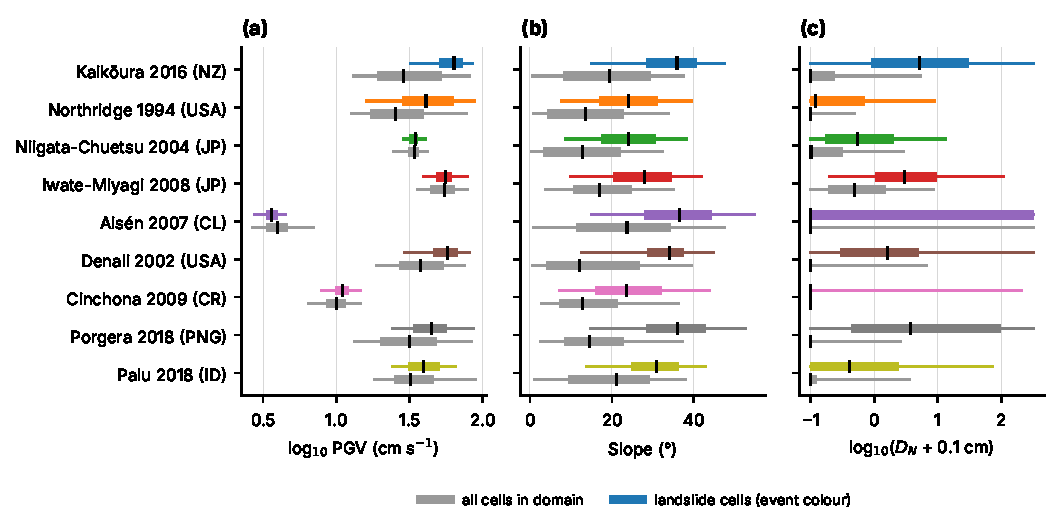
\includegraphics[width=\textwidth]{figS1_covariate_shift.pdf}
\caption{Distribution of (a) $\log_{10}$PGV, (b) slope and (c) $\log_{10}(D_N+0.1)$ over all domain cells (grey, weighted to the full domain) and over landslide cells (event colour). Thick bars span the interquartile range, thin bars the 5--95\% range, ticks mark medians.}\label{fig:shift}
\end{figure}

\section{Global logistic regression under low shaking}\label{sec:supp_lr}
Coefficients of the global LR (predictors $\log_{10}$PGV, slope, $\log_{10}$PGV$\times$slope, relief/100~m) fitted on the eight non-target events were $(-3.14, -0.066, 0.119, -0.74)$ with intercept $-2.17$ when Ays\'en was held out, $(-3.16, -0.173, 0.181, -0.65)$ with intercept $-2.20$ when Cinchona was held out, and $(-0.45, 0.045, 0.042, -0.75)$ with intercept $-6.01$ when Kaik\={o}ura was held out. The derivative of the log-odds with respect to slope, $\beta_{s}+\beta_{sv}\log_{10}\mathrm{PGV}$, becomes negative for PGV below $10^{0.066/0.119}\approx3.6$~cm\,s$^{-1}$ and $10^{0.173/0.181}\approx9.0$~cm\,s$^{-1}$ in the first two fits. The median ShakeMap PGV is 3.95~cm\,s$^{-1}$ over the Ays\'en domain and 10.1~cm\,s$^{-1}$ over the Cinchona domain, compared with 26--55~cm\,s$^{-1}$ in the other events. At Ays\'en, 95.4\% of cells have PGV below the first percentile of the training data.

\section{Gaussian tile random effect}\label{sec:supp_re}
In this alternative to the quasi-posterior of Eq.~(5) of the main text, the log-odds of cell $i$ in mapped tile $t$ are $m_i+b+u_t$ with $u_t\sim\mathcal{N}(0,\sigma_u^2)$. The tile likelihood is integrated over $u_t$ by an exact discrete Gaussian convolution of the tile log-likelihood on a grid of spacing 0.025 log-odds units; this was verified against brute-force numerical integration to eight significant digits. $\sigma_u$ and the conditional event offsets of the other events were estimated jointly by profile likelihood from their out-of-sample scores ($\hat\sigma_u=2.0$--$2.25$), and $\mu$ and $\tau$ of the prior were taken from these conditional offsets. The probability that an unmapped tile contains a landslide, needed for the selection term, was likewise averaged over $u_t$. Table~4 of the main text reports the results.

\section{Few-shot updating per event}
\begin{table}[ht]\centering\small
\caption{Per-event results of full HiPhyBoost updating (quasi-posterior with selection term): median $|\log_2 E/O|$ over 30 tile draws and coverage of the 90\% interval of the landslide total in the unmapped area. Niigata-Chuetsu has too few tiles for $k=40$.}\label{tab:perevent}
\begin{tabular}{lrrrrrrrr}\toprule
 & \multicolumn{4}{c}{$|\log_2 E/O|$} & \multicolumn{4}{c}{90\% coverage}\\\cmidrule(lr){2-5}\cmidrule(lr){6-9}
Event & $k$=1 & 5 & 10 & 40 & $k$=1 & 5 & 10 & 40\\\midrule
Kaik\={o}ura 2016 (NZ) & 0.65 & 0.47 & 0.51 & 0.36 & 0.90 & 0.77 & 0.57 & 0.63\\
Northridge 1994 (USA) & 0.50 & 0.55 & 0.46 & 0.43 & 1.00 & 0.87 & 0.80 & 0.73\\
Niigata-Chuetsu 2004 (JP) & 1.01 & 0.39 & 0.22 & -- & 0.60 & 0.63 & 0.67 & --\\
Iwate-Miyagi 2008 (JP) & 0.35 & 0.40 & 0.34 & 0.45 & 1.00 & 0.90 & 0.97 & 0.50\\
Ais\'{e}n 2007 (CL) & 0.68 & 0.45 & 0.34 & 1.15 & 1.00 & 1.00 & 1.00 & 0.80\\
Denali 2002 (USA) & 4.70 & 3.44 & 2.79 & 1.97 & 0.00 & 0.00 & 0.00 & 0.07\\
Cinchona 2009 (CR) & 3.01 & 0.78 & 0.48 & 0.64 & 0.20 & 0.60 & 0.73 & 0.23\\
Porgera 2018 (PNG) & 2.48 & 1.40 & 1.20 & 0.78 & 1.00 & 0.97 & 0.90 & 0.83\\
Palu 2018 (ID) & 0.63 & 0.53 & 0.66 & 0.52 & 0.90 & 0.93 & 0.87 & 0.53\\
\bottomrule\end{tabular}\end{table}


\section{Reliability diagrams}
\begin{figure}[h]\centering
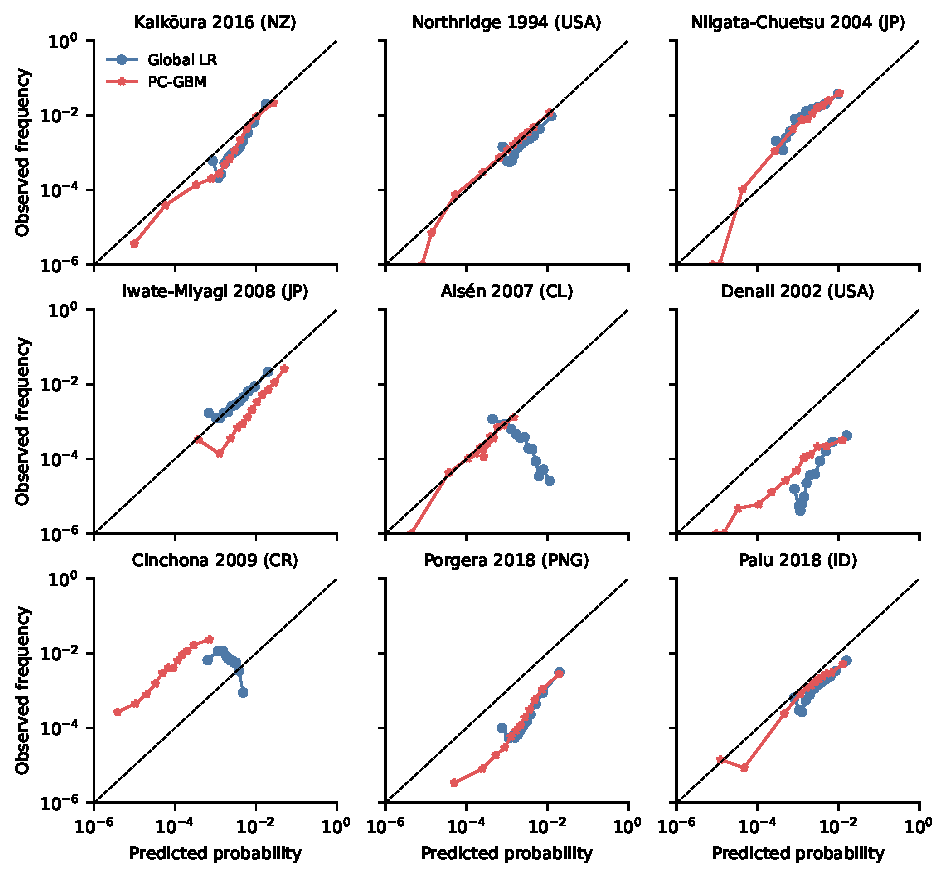
\includegraphics[width=\textwidth]{fig4_reliability.pdf}
\caption{Reliability diagrams of transferred global LR and PC-GBM models for each held-out event (log--log axes; predictions grouped into 12 quantile bins). Points above the diagonal indicate underprediction, below the diagonal overprediction.}\label{fig:reliability}
\end{figure}

\section{Full metrics of Experiment 1}
{\small\begin{longtable}{llrrrrrr}
\caption{All performance metrics of Experiment~1. AP lift: average precision divided by prevalence; BSS: Brier skill score relative to a forecast that knows the true prevalence; $E/O$: expected over observed landslide cells; slope and intercept: logistic calibration of outcomes on predicted log-odds.}\label{tab:full}\\
\toprule Event & Model & AUC & AP lift & BSS & $E/O$ & Cal. slope & Cal. int.\\\midrule\endhead
Kaik\={o}ura 2016 (NZ) & Physics (Jibson 2000) & 0.883 & 9.59 & -1.637 & 8.28 & 0.36 & -3.61\\
Kaik\={o}ura 2016 (NZ) & Physics-logit & 0.861 & 9.20 & 0.007 & 1.5 & 2.19 & 5.81\\
Kaik\={o}ura 2016 (NZ) & Global LR & 0.826 & 9.91 & 0.009 & 1.63 & 1.53 & 2.12\\
Kaik\={o}ura 2016 (NZ) & GBM & 0.894 & 7.48 & 0.007 & 0.691 & 1.14 & 1.15\\
Kaik\={o}ura 2016 (NZ) & PC-GBM & 0.887 & 9.24 & 0.010 & 1.5 & 1.07 & -0.15\\
Kaik\={o}ura 2016 (NZ) & PC-GBM (local CV) & 0.934 & 16.79 & 0.017 & 1.03 & 0.90 & -0.46\\
\midrule
Northridge 1994 (USA) & Physics (Jibson 2000) & 0.715 & 3.61 & -0.361 & 1.88 & 0.22 & -3.56\\
Northridge 1994 (USA) & Physics-logit & 0.756 & 3.36 & 0.002 & 1.14 & 1.00 & -0.16\\
Northridge 1994 (USA) & Global LR & 0.723 & 3.94 & 0.002 & 1.44 & 1.03 & -0.17\\
Northridge 1994 (USA) & GBM & 0.788 & 2.43 & -0.029 & 1.04 & 0.43 & -3.00\\
Northridge 1994 (USA) & PC-GBM & 0.814 & 5.02 & 0.004 & 0.937 & 0.96 & -0.13\\
Northridge 1994 (USA) & PC-GBM (local CV) & 0.893 & 8.92 & 0.009 & 1.01 & 0.97 & -0.12\\
\midrule
Niigata-Chuetsu 2004 (JP) & Physics (Jibson 2000) & 0.763 & 2.96 & -0.127 & 1.18 & 0.22 & -2.75\\
Niigata-Chuetsu 2004 (JP) & Physics-logit & 0.767 & 2.94 & -0.005 & 0.175 & 1.50 & 4.74\\
Niigata-Chuetsu 2004 (JP) & Global LR & 0.750 & 3.27 & -0.002 & 0.197 & 0.82 & 0.64\\
Niigata-Chuetsu 2004 (JP) & GBM & 0.774 & 2.84 & -0.005 & 0.123 & 0.72 & 0.43\\
Niigata-Chuetsu 2004 (JP) & PC-GBM & 0.788 & 3.21 & -0.001 & 0.226 & 0.88 & 0.86\\
Niigata-Chuetsu 2004 (JP) & PC-GBM (local CV) & 0.809 & 3.19 & 0.010 & 1 & 0.73 & -1.03\\
\midrule
Iwate-Miyagi 2008 (JP) & Physics (Jibson 2000) & 0.777 & 4.06 & -1.295 & 7.76 & 0.40 & -3.59\\
Iwate-Miyagi 2008 (JP) & Physics-logit & 0.764 & 3.86 & 0.004 & 0.73 & 1.79 & 4.59\\
Iwate-Miyagi 2008 (JP) & Global LR & 0.750 & 4.56 & 0.008 & 0.978 & 0.96 & -0.16\\
Iwate-Miyagi 2008 (JP) & GBM & 0.796 & 4.58 & 0.008 & 1.19 & 1.00 & -0.17\\
Iwate-Miyagi 2008 (JP) & PC-GBM & 0.833 & 5.60 & -0.010 & 2.58 & 1.20 & -0.24\\
Iwate-Miyagi 2008 (JP) & PC-GBM (local CV) & 0.834 & 5.74 & 0.008 & 1.03 & 0.80 & -0.92\\
\midrule
Ais\'{e}n 2007 (CL) & Physics (Jibson 2000) & 0.609 & 1.66 & -27.005 & 82.9 & 0.11 & -6.69\\
Ais\'{e}n 2007 (CL) & Physics-logit & 0.739 & 2.53 & -0.318 & 16.8 & 1.55 & -0.37\\
Ais\'{e}n 2007 (CL) & Global LR & 0.247 & 0.60 & -0.068 & 10.8 & -0.81 & -13.05\\
Ais\'{e}n 2007 (CL) & GBM & 0.639 & 1.64 & -0.000 & 1.12 & 0.99 & -0.12\\
Ais\'{e}n 2007 (CL) & PC-GBM & 0.760 & 3.34 & 0.000 & 1.11 & 0.99 & -0.12\\
Ais\'{e}n 2007 (CL) & PC-GBM (local CV) & 0.826 & 3.90 & -0.000 & 1.04 & 0.98 & -0.11\\
\midrule
Denali 2002 (USA) & Physics (Jibson 2000) & 0.831 & 3.92 & -61.682 & 228 & 0.31 & -6.91\\
Denali 2002 (USA) & Physics-logit & 0.845 & 3.82 & -0.363 & 41.7 & 1.65 & -0.32\\
Denali 2002 (USA) & Global LR & 0.830 & 4.26 & -0.412 & 39.5 & 1.65 & -0.32\\
Denali 2002 (USA) & GBM & 0.850 & 4.65 & -0.328 & 21.8 & 1.55 & -0.29\\
Denali 2002 (USA) & PC-GBM & 0.805 & 3.44 & -0.201 & 23.4 & 1.53 & -0.26\\
Denali 2002 (USA) & PC-GBM (local CV) & 0.883 & 9.15 & 0.000 & 0.999 & 1.00 & -0.09\\
\midrule
Cinchona 2009 (CR) & Physics (Jibson 2000) & 0.559 & 1.47 & -0.246 & 0.934 & 0.13 & -3.33\\
Cinchona 2009 (CR) & Physics-logit & 0.734 & 2.52 & -0.001 & 0.31 & 0.78 & -0.12\\
Cinchona 2009 (CR) & Global LR & 0.397 & 0.74 & -0.004 & 0.365 & -0.40 & -7.51\\
Cinchona 2009 (CR) & GBM & 0.780 & 3.94 & -0.006 & 0.0184 & 0.86 & 2.84\\
Cinchona 2009 (CR) & PC-GBM & 0.774 & 2.94 & -0.006 & 0.0213 & 0.82 & 2.37\\
Cinchona 2009 (CR) & PC-GBM (local CV) & 0.812 & 4.96 & 0.008 & 0.982 & 0.81 & -0.79\\
\midrule
Porgera 2018 (PNG) & Physics (Jibson 2000) & 0.885 & 9.77 & -9.588 & 35.9 & 0.35 & -5.02\\
Porgera 2018 (PNG) & Physics-logit & 0.892 & 9.82 & -0.037 & 8.77 & 1.38 & -0.23\\
Porgera 2018 (PNG) & Global LR & 0.847 & 11.57 & -0.101 & 10.1 & 1.42 & -0.26\\
Porgera 2018 (PNG) & GBM & 0.876 & 8.55 & -0.052 & 5.56 & 1.29 & -0.21\\
Porgera 2018 (PNG) & PC-GBM & 0.872 & 9.05 & -0.097 & 8.84 & 1.40 & -0.25\\
Porgera 2018 (PNG) & PC-GBM (local CV) & 0.934 & 18.67 & 0.004 & 1.02 & 0.98 & -0.10\\
\midrule
Palu 2018 (ID) & Physics (Jibson 2000) & 0.742 & 3.00 & -1.974 & 8.69 & 0.19 & -4.58\\
Palu 2018 (ID) & Physics-logit & 0.762 & 3.03 & -0.001 & 2.07 & 1.10 & -0.19\\
Palu 2018 (ID) & Global LR & 0.733 & 3.34 & -0.006 & 2.44 & 1.13 & -0.20\\
Palu 2018 (ID) & GBM & 0.790 & 3.86 & 0.002 & 0.816 & 0.94 & -0.12\\
Palu 2018 (ID) & PC-GBM & 0.730 & 2.49 & -0.004 & 1.89 & 1.08 & -0.17\\
Palu 2018 (ID) & PC-GBM (local CV) & 0.838 & 4.61 & 0.002 & 0.97 & 0.96 & -0.12\\
\bottomrule
\end{longtable}
}

\section{The 38 earthquakes of the global extension}
{\small\begin{longtable}{lrrrcrrrrrl}
\caption{The 38 earthquakes of the global extension (ordered by year). Landslide cells and domain area on the 30~m grid; inventory type A = polygons (areas), P = points; ShakeMap stations; antecedent precipitation relative to its 1981--2010 climatology; leave-one-event-out AUC of PC-GBM and HiPhyBoost; HiPhyBoost event offset from the fit to all 38 events; source: ScienceBase item identifier of the inventory in the USGS repository (Schmitt et al. 2017; https://www.sciencebase.gov/catalog/item/<identifier>) or GNS Science (Kaik\={o}ura).}\label{tab:global}\\
\toprule Event & M & Landslide cells & km$^2$ & Inv. & Stations & Rain ratio & AUC PC-GBM & AUC HiPhy & $b_e$ & Source\\\midrule\endhead
San Fernando 1971 & 6.6 & 387 & 482 & P & 113 & 0.23 & 0.623 & 0.620 & -0.68 & \texttt{\scriptsize 5874cc26e4b0a829a320bbd4}\\
Guatemala 1976 & 7.5 & 6\,136 & 5\,265 & A & 0 & 0.59 & 0.691 & 0.698 & +0.23 & \texttt{\scriptsize 5874b3d4e4b0a829a320bb73}\\
Southern Italy 1980 & 6.9 & 68 & 11\,265 & P & 27 & 1.91 & 0.654 & 0.647 & -4.18 & \texttt{\scriptsize 5b6b2a35e4b006a11f779851}\\
Livermore 1980 & 5.8 & 105 & 908 & P & 12 & 1.20 & 0.683 & 0.697 & -0.54 & \texttt{\scriptsize 5874bdede4b0a829a320bbca}\\
Mammoth Lakes 1980 & 6.1 & 4\,024 & 2\,411 & A & 0 & 1.08 & 0.873 & 0.876 & +1.68 & \texttt{\scriptsize 5874bd42e4b0a829a320bbb9}\\
Coalinga 1983 & 6.7 & 3\,881 & 1\,856 & A & 48 & 2.37 & 0.791 & 0.798 & +1.76 & \texttt{\scriptsize 5874a164e4b0a829a320bb10}\\
San Salvador 1986 & 5.7 & 267 & 368 & P & 0 & 0.77 & 0.670 & 0.671 & +0.89 & \texttt{\scriptsize 5874ccaae4b0a829a320bbd9}\\
Loma Prieta 1989 & 6.9 & 1\,732 & 1\,905 & P & 101 & 2.41 & 0.686 & 0.694 & +0.21 & \texttt{\scriptsize 5874bd02e4b0a829a320bbb4}\\
Valle de la Estrella 1991 & 7.6 & 1\,643 & 2\,021 & A & 13 & 0.83 & 0.727 & 0.799 & -0.68 & \texttt{\scriptsize 5874bcc2e4b0a829a320bbaf}\\
Northridge 1994 (USA) & 6.7 & 10\,925 & 4\,377 & A & 185 & 0.41 & 0.809 & 0.831 & +1.38 & \texttt{\scriptsize 58595917e4b03639a6025f30}\\
Kobe 1995 & 6.9 & 2\,158 & 175 & A & 20 & 0.95 & 0.754 & 0.777 & +1.88 & \texttt{\scriptsize 58b538b7e4b01ccd54fddf59}\\
Central Italy 1997 & 6.0 & 176 & 9\,230 & P & 25 & 0.52 & 0.861 & 0.868 & -2.17 & \texttt{\scriptsize 5b6b075ee4b006a11f77930e}\\
Jueili 1998 & 5.7 & 847 & 1\,000 & A & 0 & 0.84 & 0.654 & 0.684 & +0.38 & \texttt{\scriptsize 5b5a20eee4b0610d7f4dcc52}\\
San Miguel 2001 & 7.7 & 134 & 8\,175 & P & 10 & 0.35 & 0.754 & 0.761 & -2.96 & \texttt{\scriptsize 5874cce7e4b0a829a320bbde}\\
Denali 2002 (USA) & 7.9 & 1\,579 & 15\,748 & A & 24 & 1.13 & 0.813 & 0.848 & -2.48 & \texttt{\scriptsize 5874a336e4b0a829a320bb15}\\
Lefkada 2003 & 6.3 & 252 & 223 & A & 9 & 1.10 & 0.864 & 0.878 & -0.02 & \texttt{\scriptsize 5874bc90e4b0a829a320bbaa}\\
Niigata-Chuetsu 2004 (JP) & 6.6 & 4\,860 & 410 & A & 448 & 1.17 & 0.799 & 0.800 & +2.45 & \texttt{\scriptsize 5874bd79e4b0a829a320bbbe}\\
Kashmir 2005 & 7.6 & 2\,929 & 4\,407 & A & 0 & 0.82 & 0.737 & 0.737 & -2.62 & \texttt{\scriptsize 5895dabfe4b0fa1e59bc788f}\\
Kiholo Bay 2006 & 6.7 & 379 & 229 & A & 23 & 0.97 & 0.872 & 0.864 & +0.14 & \texttt{\scriptsize 5874bb8de4b0a829a320bb9f}\\
Pisco 2007 & 8.0 & 271 & 21\,652 & P & 13 & 0.52 & 0.806 & 0.825 & -3.57 & \texttt{\scriptsize 5b5f3190e4b006a11f66e491}\\
Ais\'{e}n 2007 (CL) & 6.2 & 512 & 1\,247 & A & 0 & 0.74 & 0.654 & 0.691 & +0.84 & \texttt{\scriptsize 586fe5a7e4b01a71ba0c5f06}\\
Iwate-Miyagi 2008 (JP) & 6.9 & 4\,093 & 777 & A & 449 & 0.93 & 0.827 & 0.827 & +0.98 & \texttt{\scriptsize 5b59ec98e4b0610d7f4da850}\\
Wenchuan 2008 & 7.9 & 197\,160 & 77\,832 & A & 421 & 0.98 & 0.859 & 0.859 & +0.48 & \texttt{\scriptsize 586d7498e4b0f5ce109fc93b}\\
Cinchona 2009 (CR) & 6.1 & 4\,743 & 637 & A & 0 & 1.19 & 0.785 & 0.783 & +2.88 & \texttt{\scriptsize 61ead71bd34e8b818ad9f44b}\\
Haiti 2010 & 7.0 & 20\,702 & 3\,741 & A & 4 & 2.25 & 0.827 & 0.848 & +1.28 & \texttt{\scriptsize 585872dce4b0e40e53c241e1}\\
Tohoku-Oki 2011 & 9.1 & 3\,375 & 28\,934 & A & 1204 & 1.02 & 0.563 & 0.551 & -1.58 & \texttt{\scriptsize 5874a54be4b0a829a320bb2a}\\
Western Sichuan 2013 & 6.6 & 15\,278 & 5\,490 & P & 3 & 0.98 & 0.743 & 0.792 & +0.66 & \texttt{\scriptsize 59442c43e4b062508e3231be}\\
Gansu 2013 & 5.9 & 2\,169 & 320 & A & 2 & 1.28 & 0.705 & 0.655 & +2.64 & \texttt{\scriptsize 59442b04e4b062508e3231af}\\
Sichuan-Yunnan-Guizhou Region 2014 & 6.2 & 1\,024 & 363 & A & 0 & 1.20 & 0.747 & 0.772 & +0.91 & \texttt{\scriptsize 594428d4e4b062508e32319f}\\
Nepal 2015 & 7.8 & 20\,630 & 24\,517 & A & 2 & 1.08 & 0.795 & 0.822 & -0.80 & \texttt{\scriptsize 61f040e1d34e8b818adc3251}\\
Norcia 2016 & 6.6 & 349 & 4\,203 & P & 310 & 0.82 & 0.859 & 0.876 & -1.16 & \texttt{\scriptsize 5b6b2201e4b006a11f7795c3}\\
Kaik\={o}ura 2016 (NZ) & 7.8 & 28\,474 & 10\,832 & P & 227 & 1.05 & 0.892 & 0.917 & +0.62 & \texttt{\scriptsize GNS}\\
Visso 2016 & 6.1 & 204 & 673 & P & 87 & 0.82 & 0.755 & 0.800 & -0.46 & \texttt{\scriptsize 5b6b1177e4b006a11f7793ea}\\
Milin 2017 & 6.4 & 762 & 1\,755 & A & 0 & 0.94 & 0.770 & 0.754 & -1.14 & \texttt{\scriptsize 5f4d1e9c82ce4c3d12318d43}\\
Porgera 2018 (PNG) & 7.5 & 10\,455 & 24\,306 & A & 1 & 1.56 & 0.884 & 0.918 & -0.89 & \texttt{\scriptsize 61f04680d34e8b818adc32a8}\\
Palu 2018 (ID) & 7.5 & 7\,007 & 3\,665 & P & 0 & 1.04 & 0.729 & 0.776 & +0.47 & \texttt{\scriptsize 61f196a1d34e8b818add4fdf}\\
Lombok 2018 & 6.9 & 9\,265 & 1\,797 & A & 0 & 1.00 & 0.662 & 0.678 & +2.51 & \texttt{\scriptsize 5ef2514782ced62aaae3bcab}\\
Mesetas 2019 & 5.7 & 837 & 3\,101 & A & 0 & 1.47 & 0.950 & 0.927 & +0.66 & \texttt{\scriptsize 61ead1f5d34e8b818ad9f37f}\\
\bottomrule
\end{longtable}
}

\section{Zero-shot priors conditioned on event covariates}
\begin{table}[ht]\centering\small
\caption{Zero-shot priors for the event offset in the 38-event leave-one-event-out analysis. LPD: mean log predictive density of the held-out offset (nats); gain relative to the unconditional prior with paired Wilcoxon $p$ and permutation $p$ (200 random permutations of the covariate vectors among events); coverage of the 90\% interval for the landslide total; median interval width (ratio of bounds) and median error factor of the median forecast.}\label{tab:offreg}
\resizebox{\textwidth}{!}{\begin{tabular}{llrrrrrrr}\toprule
Covariates & Available & LPD & Gain & $p$ & $p_{\mathrm{perm}}$ & Coverage & Width & Error\\\midrule
None (unconditional prior) &  & -2.03 & -- & -- & -- & 33/38 & 364 & 2.9\\
F1: Mw, depth, mechanism, ShakeMap stations & forecast & -1.86 & +0.18 & 0.038 & 0.005 & 33/38 & 132 & 3.2\\
F2: PDSI, rain ratio, mean annual rain & forecast & -2.08 & -0.04 & 0.293 & 0.945 & 33/38 & 342 & 3.1\\
F3: F1 + F2 & forecast & -1.87 & +0.16 & 0.048 & 0.005 & 34/38 & 137 & 3.3\\
P1: inventory type, mapping extent, year & post-event & -1.99 & +0.04 & 0.153 & 0.030 & 33/38 & 245 & 3.6\\
P2: P1 + domain area & post-event & -1.83 & +0.20 & 0.010 & 0.005 & 36/38 & 120 & 3.4\\
P3: F3 + P2 & post-event & -1.85 & +0.18 & 0.067 & 0.005 & 35/38 & 121 & 3.3\\
\bottomrule\end{tabular}}\end{table}



\end{document}
